\documentclass[msc,pdftex]{Estilos/coppe}
%other options
%doublespacing HAHHAHAHAHAH


\usepackage{enumitem}
\usepackage{multicol}
\usepackage[T1]{fontenc}
\usepackage[utf8x]{inputenc}
\PrerenderUnicode{ě} %for bibitem beholavek2002
\usepackage{verbatim}
\setcounter{secnumdepth}{4} %numbering subsubsections
\setcounter{tocdepth}{4} %subsubsections in table of contents
\usepackage[ruled,vlined,linesnumbered]{algorithm2e}

\usepackage{amsmath,amssymb}
\usepackage{relsize}
\usepackage{graphicx}
\usepackage{courier}
\usepackage{todonotes}

\usepackage{booktabs}

% não deixa figura mudar de seção e
% habilita o commando \FloatBarrier
\usepackage[section]{placeins}

%subcaption and subfigure
\usepackage{subfig}
\usepackage{caption}

%\renewcommand\thesubfigure{ (\alph{subfigure})}

%apud citation style
\newcommand{\apudp}[2]{(\citeauthor{#1},\space\citeyear{#1},\space as cited in \citeauthor{#2},\space\citeyear{#2})}
%\newcommand{\apud}[2]{\citeauthor{#1}\space (as cited in \citeauthor{#2},\space\citeyear{#2})}

%full centered cell
\newcommand{\specialcell}[2][c]{%
  \begin{tabular}[#1]{@{}c@{}}#2\end{tabular}}
\usepackage{multirow}
%\usepackage{array}

\usepackage{longtable}

\usepackage[hyphens]{url}
\usepackage{hyperref}
\usepackage{lmodern}
\usepackage{rotating}
\usepackage{tikz}
\usepackage{pgfplots}
\usepackage{pgfplotstable}
\usepackage{ucs}
\usepackage{changepage}
\usepgflibrary{fpu}
\usetikzlibrary{shapes.multipart, mindmap, arrows, positioning}

%preventing widow and orphan lines
\widowpenalty=10000
\clubpenalty=10000
\postdisplaypenalty=10000

%footnote in verty bottom
\usepackage[bottom]{footmisc}

\usepackage{float}

%to include pdfs in the doc
\usepackage{pdfpages} 

%\addto{\captionsenglish}{\renewcommand{\bibname}{Referências Bibliográficas}}


% to make editor notes
%\usepackage[show]{ed}

\makelosymbols
\makeloabbreviations

\pgfplotsset{compat=1.12}

%%%%%%%%%%%%%%%% ROUBADO DO MANGELI
% Citacao direta com mais de 3 linhas - ABNT NBR 10520/2002 - 5.3
\newcommand{\ABNTEXfontereduzida}{\footnotesize}
\newlength{\ABNTEXcitacaorecuo}% recuo de 4 cm da margem esquerda
% \ifthenelse{\equal{\ABNTEXistwocolumn}{true}}{%
%   \setlength{\ABNTEXcitacaorecuo}{1.8cm}
% }{% else
%   \setlength{\ABNTEXcitacaorecuo}{4cm}
% }
\setlength{\ABNTEXcitacaorecuo}{4cm}

\newenvironment*{citacao}[1][default]{%
   \list{}%
   \ABNTEXfontereduzida%
   \addtolength{\leftskip}{\ABNTEXcitacaorecuo}%
   \item[]%
   %\begin{singlespacing}%
   \singlespacing
   \ifthenelse{\not\equal{#1}{default}}{\itshape\selectlanguage{#1}}{}%
 }{%
   %\end{singlespacing}%
   \endlist}%
% ---



\begin{document}


	\title{An ontology of board games based on the MDA framework}
	\foreigntitle{Uma ontologia de jogos de tabuleiro fundamentada no framework MDA}
	\author{Joshua Silveira}{Kritz}
	\advisor{Prof.}{Geraldo Bonorino}{Xexéo}{D.Sc.}
	%\advisor{Prof.}{Nome do Segundo Orientador}{Sobrenome}{Ph.D.}
	%\advisor{Prof.}{Nome do Terceiro Orientador}{Sobrenome}{D.Sc.}
	
	\examiner{Prof.}{Geraldo Bonorino Xexéo}{D.Sc.}
	\examiner{Prof.}{Tadeu Moreira de Classe}{D.Sc.}
	\examiner{Prof.}{Renata Mendes de Araujo}{D.SC.}
	\examiner{Prof.}{Jano Moreira de Souza}{D.SC.}
	\department{PESC}
	\date{03}{2020}
	
	
	
	
	\keyword{games}
	\keyword{game models}
	\keyword{boardgames}
	\keyword{ontology}
	\keyword{conceptual modeling}
	
	\maketitle
	\frontmatter
	
	\dedication{To my first fan \\ Mom}


	\chapter*{Agradecimentos}

Gostaria de agradecer primeiramente ao meu orientador Geraldo Bonorino Xexéo. Por ter me dado essa incrível oportunidade que é estudar jogos. Por ter me apoiado nesta jornada e puxado minha orelha quando necessário. Mas principalmente por confiar em mim e nas minhas habilidades.

Aos meus companheiros do LUDES pela amizade e pelas reuniões animadissimas e altamente instrutivas e esclarecedoras. \#partiuJogar!

Para minha família meus mais profundos agradecimentos por terem sempre torcido por mim e me apoiado nas minhas loucuras. Em especial ao meu Pai e minha Mãe que nunca me deixarão desistir da minha insessante busca por conhecimento. 

A Patrícia Musmanno, por ter sido uma companheira maravilhosa nesta jornada. Me apoiar na busca dos meus sonhos, e me abraçar nos momentos difíceis. Você tornou esta jornada mais alegre e agradável.

Um agradecimento especial ao Prof. Milton Ramirez, que me acolheu no ínicio da minha jornada do ensino superior. Me ensinou quase tudo que sei sobre programação e computação. Obrigado por ter me apoiado e guiado.

A Lucas Andrade, por ser um amigo que sempre esteve ao meu lado. E por ajudar na super ágil revisão desta dissertação. Obrigado pelas risadas e curiosidades.

Aos amigos da Casa do Goblin que aceitaram participar do Grupo Focal, Adalberto Taconi, Andreza Farias Henrique, Ddesir\'{e} Taconi, Fransisco De Paula, Jorge Lu\'{i}s Rocha, Leandro Pinto, Rafael Romualdo,Sabrina Do Valle, Thaila Vega, Nath Bras. Em especial a Sanderson Gomes Virgolino, pela parceria e incríveis trocas de ideias sobre o mundo dos boardgames.

Um agradecimento ao querido Wagner Santos, por ter me apresentado ao Xexeo. Se não fosse por isso, jamais teria me aventurado na academia de jogos.

Ao CNPq - Conselho Nacional de Desenvolvimento Científico e Tecnológico - agradeço por ter prestado auxílio financeiro para o desenvolvimento do meu Mestrado. 
	\begin{abstract}

Esta dissertação utiliza de teorias muito bem fundamentadas na literatura para dar um primeiro passo na criação de uma base de conhecimento sobre jogos de tabuleiro. Produzindo assim uma ontologia fundamentada sobre o framework MDA \citet{Hunicke2004} e criada sobre os preceitos da UFO \citet{guizzardi_ontological_2005}. Para isso se investiga de forma mais profunda o que são mecânicas, dinâmicas e estéticas, utilizando tanto conhecimento prático de pessoas envolvidas quanto bases teóricas fortes como \citet{ekman_are_basic_emotions_nodate} e \citet{dillon_way_2010}. Finalmente produzindo um artefato a ser utilizado para melhorar o entendimento de jogos de tabuleiro.

\end{abstract}


	\begin{foreignabstract}

This dissertation uses theories highly recognized in the literature to take a first step in creating a knowledge base about board games. Thus producing an ontology based on the MDA framework \citet{Hunicke2004} and created upon the precepts of UFO \citet{guizzardi_ontological_2005}. For this it investigates more deeply what mechanics, dynamics and aesthetics are, using as much practical knowledge of the people involved as strong theoretical basis such as \citet{ekman_are_basic_emotions_nodate} and \citet{dillon_way_2010}. Finally producing an artifact to be used to improve the understanding of board games.

\end{foreignabstract}

	
	\tableofcontents
    \listoffigures
    \listoftables
    \printlosymbols
    \printloabbreviations
	
	\mainmatter
	
	\chapter{Beginings}

This section presents this dissertation's proposal and introduce the main ideas that will be used in it's construction. It contains the motivations as well as a broad spectrum view of this work. Whilst introducing core concepts that will be used in this dissertation.

\section{Why games?}

Nowadays we live surrounded by games. There are games in smart-phones that are played while we come and go to our everyday tasks, games in our houses, in computers and even where there seems to be no games, there are people talking about games.

Financially, games are a big industry. The revenue of many video game companies are in the score of billions of dollars. \citet{babb2013comparing} evaluates diverse companies and games, giving a good illustration of this big industry. Only the US video game market is worth over 20 billion dollars. A single game, World of Warcraft, had almost 1 billion dollars revenue by itself. All of this before 2011, when today this market has only increased. This shows how big games are in the modern world, which enforces why we should study them deeply.

Games are also becoming present on education. Game-based learning became a very popular approach to teaching in many levels of education. In \citet{hainey2016systematic} the sheer amount of practical experiences found is enough to show that games are a part of education in the twentieth century.

One can guess that, if games are so entwined in our daily lives, there will be a great understanding of them, of what games are, how games are made, what means to play a game. Surprisingly that is not true. Studies in games have a great amount of disagreement. Many aspects of games are met with different opinions among scholars. To begin with, there is no commonly accepted definition of the term game. 

Many researchers addressed the problem of finding a definition \citep{jarvinen2009games,salen2004rules,crawford1984art,schell2014art,juul2010game} but they could not agree on a single definition. Each of them pursued very different paths in their search for understanding, thus each defined games in their own way. Although there is some common ground between some of those definitions. \cite{salen2004rules} systematically compared most definitions from previous works and concluded there was no true agreement between them. \cite{wittgenstein_philosophical_2009} went further to state that there is no possible definition, ``game is a concept with blurred edges''. Such is the hardship of finding a definition for games.

Other aspects of games share this multitude of opinions. Game design or how to make games is a subject that presents a variety of ideas and models for its understanding. Although there are more common parts and shared ideas through many researches this subject is far from a global complete knowledge. There are many other questions pertaining games that remain without a completely accepted answer. Such as `why do people play games?', `how do people react to games?', `how do people behave in games?'.

In light of such confusion and dissent. The purpose of this work is to extend current understanding of what games are made of, of which parts compose this complex and intriguing whole. Hopefully, this will bring us closer to completely understanding games. At least it should provide a tool for researchers and designers that wish to adventure in the games domain to start to understand what it is. Therefore, this is an attempt to create a boardgame ontology using the ontological principles of UFO \citep{guizzardi_ontological_2005}. It will provide the foundation for a human oriented ontology. This ontology is structured upon the MDA framework \citep{Hunicke2004} as it is simple and widely accepted. 

This dissertations focus its efforts in boardgames, this is due the author's experience, but also because the boardgame industry is increasing rapidly over the past decade and becoming a very expressive part of the daily lives in many countries. In a market report, done by Grand View Research \footnote{\url{https://www.grandviewresearch.com/industry-analysis/playing-cards-board-games-market} Accessed in 12/03/2020}, the boardgame market size was almost 12 billion dollars, with an expected increase of 8,79\% over the next six years. It still does not compete with video games, but this growth implies that boardgames are becoming more and more important over the years and must be addressed accordingly.
\section{Research Problem}

The research problem addressed in this dissertation is represented by the following research questions:
\begin{enumerate}
    \item {What work have been done about game ontologies?}
    \item {What means there are to describe the boardgame domain using an ontology?}
    \item {In what ways an ontology can be composed to better represent the challenges on board game domain?}
    \item {How to create a domain ontology of boardgames focused on humans rather than machines?}
    \item{Do this ontology provides better understanding of the boardgames domain?}
\end{enumerate}
\section{Concepts}
In this section some important concepts used in this work are exposed and explained in accord to their meaning to this dissertation. To be clear about what they mean whenever they are used. As it is not in the scope of this work there will be no rigid definition of the word Game. When looking into the definitions given by the many authors mentioned in section 1.1 it is possible to understand what is a game to this work. 

\textbf{Boardgame} is used with the idea of a non-digital game. It does not need to have a board, it can be a game made of only cards or even a mimic game with no object, only the rules. The scope of this work does not include digital games. We use the word boardgame, instead of game, throughout this dissertation to emphasize this.

The terms, \textbf{mechanics}, \textbf{dynamics} and \textbf{aesthetics} are used with accord to their definition in the MDA framework, which is explained in the next chapter. 

\textbf{Magic Circle} is a notion first introduced in \cite{huizinga2014homo}. Although \citeauthor{huizinga2014homo} did not named it so, many scholars that further developed the concept name it as Magic Circle. \cite{salen2004rules,bateman_implicit_2015} are only a few examples. This concept develops on the idea that there is a certain boundary in reality in which a play of a game takes place and this boundary prohibits some aspects of reality to affect the game space, in other words it protects the game from the real world. The Magic Circle became very important to the studies of games and whenever mentioned throughout this work the Magic Circle significance is in accordance to the understanding given by \cite{salen2004rules}.

\textbf{World} is addressed in the modeling concept of the real world. A given world is a possible reality of facts and beings that are part of the modeled domain. In other words a world is a possible existence. An example, say that a model of families exist. One world is that Carlos, Mandy and Bob form a family while Eduardo, Sandra and Charlie form another. A second possible world is that Carlos, Eduardo and Bob from the first family while the others form the second one. 


\section{Structure of this work}

This first chapter is used to introduce the general idea of this dissertation as well as some important concepts that are used throughout it.

Chapter 2 will present a literature review, which will cover the topics of this dissertation. First it presents works that are similar to some degree to the one that will be done here. Ontologies made about the game domain, including some that were not about game specifically but about specific aspects of games. Then it establishes references used as foundation knowledge for this work, such as books, theories and ideas that were fundamental to the author's understanding of the area. Finally it introduces a review of the subjects nested in the MDA framework. That is, provides a review of works done with respect to mechanics, dynamics and aesthetics that were in accord with their definition.

The next chapter will discourse about the methodology chosen for this work, presenting and explaining the UFO and OntoUML and how they will be used to bring fruition to this ontology. It will explain the ideas of UFO and the reasoning behind the choice of it. And about why this is different from other attempts on building ontologies in the games domain. Furthermore it shows why OntoUML is a natural choice when describing an ontology founded in UFO. 

Following the methodology, chapter 4 presents the results of the research on dynamics. Using these results it is also established a vocabulary of dynamics, which is used to create the dynamics section of this ontology.

Using the background built until then, the fifth chapter summarizes the proposal of this dissertation. Thoroughly explaining what is to be done in the creation of the ontology of boardgames and why is it done so. It provides the theoretical foundation of the ontology, the core modeling choices made, their explanation and reasoning and how to use the OntoUML language to represent the concepts contained in the ontology.

Chapter 6 will then contain the implementation of the ontology in the prolog language. This is the computable form of the ontology. And this chapter covers its creation as well as functionalities and how to use it. Also covering how to evaluate improvements to this ontology.

Finally, chapter 7 concludes this work discoursing and summarizing what was done here. Also exposing how future works can improve the line of research and even create new ones.


	\chapter{What we know so far}

This chapter aims to present the knowledge and ideas used as foundation for this work, looking into similar perspectives, theory about games and presenting knowledge pertaining the methodology chosen.

\section{Game ontologies}

The whole idea of creating a ontology about games is not a novelty. There are many attempts to create such artifact, although not specifically about boardgames, each of them with their own purpose. The most known of those attempts is the Game Ontology Project (GOP) \citep{wiki:gop}, “a framework for describing, analyzing and studying games” \citep{Zagal:2008:GOP}. It  provides  a  structure  to  study  games  elements  based  on four top-level elements:  interface,  rules,  entity manipulation and goals. It  is  a  collaborative  work,  open  to  contributions, although as of 11/11/2019 its development stalled. Some of its elements can be identified in the ontology proposed in this work. Most of it in the Mechanics ontology. Those semblances are further covered in \citep{kritz_buildingOntology}. Roman,  Sandu,  and  Buraga  constructed  an  ontology  for  role-playing games (RPG) in a work inspired by GOP \citep{roman2011owl}.That work uses the OWL language to describe the ontology and intends to facilitate designers’ activities like character creation, NPC generation, simple battle system configuration, etc. A slightly more comprehensive  ontology was created in the realm of RPG \citep{dhuric2015specific}. Although  using  a  specific  game,  \cite{manaworld}, as the source of concepts, the authors claim that the resulting ontology is applicable to massively multiplayer online role-playing games (MMORPG).

More recently, GOP and MDA were also used to provide a model for innovation in digital games \citep{innov:gop:mda}. Three Hundred Mechanics is a video game oriented catalog of game mechanics, with examples \citep{300gm}. It is very comprehensive and provides five collections: Comp-grid, Procedural, Tactics, Tiny Crawl and Misc. It is maintained by a single person, but also seems to have ceased to evolve, as of 2019. In \cite{leon_z._ontology_2010} a Mobile games ontology is developed while investigating the use of UML and OCL for ontology representation. Another recent work focused in video games is \cite{parkkila_ontology_2017}, in which the authors claim that can enable interoperability between games. A Game Character Ontology developed in \cite{sacco_game_2017} provides tools to be used in the creation of game characters.

In the realm of Serious Games there are some other attempts on ontology creation. A group of researchers at Aristotle University of Thessaloniki created an ontology for exergames proposing a "unified model for the semantic representation of exergames" \citep{bamparopoulos_towards_2016} with the objective to propose standards for the research on exergames. In a different approach Tang and Hanneghan created the Game Content Model (GCM) \citep{tang_game_2011}, which is an ontology about documenting serious game design. With the objective of helping new game designers with methods and game design models. Although the main subject of GCM is not exactly the game, but game documentation, it provides great insight in taking the player into account in its model. More specifically for games in education \cite{ghannem2011defining} created a ontology for integrating games and learning processes.
\section{Background knowledge of games}

Although not defining the term game, it is important to be clear about how we understand games. About what are the paving stones for the knowledge used in this work. In such light this section discourses about many authors and their works, which compose the foundation of the view of games domain. First it is important to note that most of the references mentioned here are not specific about boardgames, some are even exclusively about video games, but nonetheless they are important to clarify the way this work look and delve into boardgames. As most of the knowledge in such references are about games in general their ideas are completely valid for boardgames. Although the specifics of how to fit these ideas in this domain was brought mostly by experience.

The most notable foundation is the MDA framework \cite{Hunicke2004}, chosen as the core structure of this dissertation. It will be explained in a section of its own given how important it is to this work.

Close to the MDA framework, but different in the way it relates the game components, is \cite{schell2014art} framework. He defines mechanics much like the MDA and aesthetics in a different but similar way. It includes the visual and sensory aspects of the game. But do not define the emotions as aesthetics and actually relates them as cause-effect. Schell does not include the dynamics in his framework, but it introduces two components, Story and technology. The former is important to understand how the narrative and the reasoning behind mechanics, impact the game. Technology is of great importance here. In Schell's framework it is the actual choice of implementation of the game. How it exists as an artifact, if it is paper and plastic objects, a book, code and data in a digital setting. The importance of it to games is that it imposes limits to the game. An example, for a game to be created for a mobile platform, it cannot have the same quality of graphics and sound as if it was to be played in a complete desktop. In a more complex comparison, Role Playing Games, which are written in books, can have a flexible set of rules, most of the time the rules are dictated by a master and aren't even written on the book. Such characteristic is difficult to obtain in digital games, as these rules needs to be pre-coded. This distinction given to the choice of technology is definitive for this work, as it is why I think worth to study a specific type of technological limitation. Of physical papers and plastic objects and a rulebook, this scope allows to better enlighten this limitations and advantages of a specific technology.

When studying games there are many facets that can be persecuted, \cite{salen2004rules} acknowledge it in their work and even used this in their framework. They termed this process of focusing in a specific facet as framing the game. According to \cite{salen2004rules} there is three possible ways to frame games, as Rules, Play and Culture, each of them focus on certain specific aspects of a game in detriment of other ones. To frame games as Rules means looking into the game as in and of itself without considering who plays the game, neither in what circumstances it happens. According to the authors ``Rules is a \textit{formal} primary schema, and focuses on the intrinsic mathematical structures of games''\citep{salen2004rules}. The Rules frame focus on the mechanics of the games. Increasing the scope of the frame there is Play, this frame begins to take into account the player of the game, what he does and how he behave, as the authors state ``Play is an \textit{experiential} primary schema and emphasizes the player's interaction with the game and other players.'' \cite{salen2004rules}. In accord with the MDA, the Play frame focus on Dynamics and the Aesthetics of the game. The broader scope of this framing is Culture, it goes beyond the game and its players to look into the social behaviour and culture surrounding the game, to the authors ``Culture is a \textit{contextual} primary schema, and highlights the cultural contexts into which any game is embedded.'' \cite{salen2004rules}. This framing is not encompassed by the MDA framework, it focus on the environment in which the game exists and how it interacts with the game, not with the game itself as does the MDA. This is an important distinction, for it provides a clear understanding of one of the boundaries of this work's scope. By using the MDA as our foundation we abide to remain in its frame, which means this work frames games in a conjunction of the Rules and Play frames.


\section{MDA framework}

The MDA framework, used as a foundation for this work, is a widely accepted model for understanding and studying games, featuring over 1000 citations in April 2018 in google scholar. 

It's name is an acronym for Mechanics, Dynamics and Aesthetics, which are the three conceptual components games are made of. The framework also presents a causal relation between those components which is the most interesting contribution of this model. The MDA framework was created to help designers, scholars and researchers. Providing a tool for decomposing games in smaller parts, that are easier to manage and understand. 

The components of the framework are defined as \autoref{tab:MDA_components_description} illustrates:
{\renewcommand{\arraystretch}{1.5}
\begin{table}[!h]
    \caption{MDA components description \citep{Hunicke2004}}
    \vspace{.5em}
    \centering
    \begin{tabular}{c|m{6cm}l|}
    Mechanics &  The particular components of the games, at the level of data representation and algorithms.\\ \cline{1-2}
    Dynamics & The run-time behaviour of the mechanics, acting on player inputs and each others' outputs over time.\\ \cline{1-2} 
    Aesthetics & Emotional responses evoked in the players.\\
    \end{tabular}
    \label{tab:MDA_components_description}
\end{table}}


Those definitions, proposed by the authors, are fitting for the their model, but if we want to apply the model thoroughly in both game design and research. Deeper understanding of each of these concepts will be very useful. Hence this work intends to create an ontology for each of them, providing a tool that increases the usability of the MDA model for Boardgames. Even with a simple ontology and the foundations for a knowledge base, the use of each component of the MDA framework will be much clearer. As of today there is a lot of controversy about mechanics and aesthetics and for dynamics there is almost no information at all. With this work I intend to deliver not only a better  understanding of each component but also a coherent connection of their information to better serve the model.

%MDA diagram
\begin{figure}[ht]
\centering

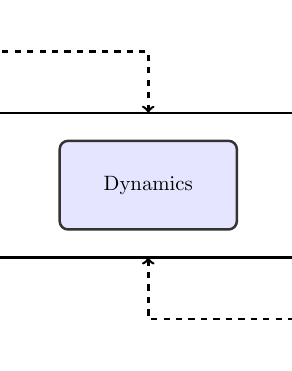
\begin{tikzpicture}[squarednode/.style={rectangle, 
					rounded corners, 
					very thick,
 					minimum width=3cm,
					minimum height=1.5cm,
					draw=black!80, 
					fill=green!10},
					squarednode2/.style={rectangle, 
					rounded corners, 
					very thick,
 					minimum width=3cm,
					minimum height=1.5cm,
					draw=black!80, 
					fill=blue!10},
					squarednode3/.style={rectangle, 
					rounded corners, 
					very thick,
 					minimum width=3cm,
					minimum height=1.5cm,
					draw=black!80, 
					fill=red!10}
					]
					
% To reduce all image, transform canvas
% forgets about image size, so 
% we need a bounding box
% This is lame, but works with Eduardo Thesis´s image (now black and white for elegance)

% don´t ask me about theses limits
% I just tried until I found which ones
%workded
\useasboundingbox (3,-2) rectangle (6,2);
\scope[transform canvas={scale=.75}]
         % Your actual drawing


%MDA nodes
\node[squarednode]  (m) [anchor = west]{Mechanics};
\node[squarednode2]  (d) [right of = m, node distance=3cm, anchor=west] {Dynamics};
\node[squarednode3]  (a) [right of = d, node distance=3cm, anchor=west] {Aesthetics};

%paths designer
%\path [-latex,  black, very thick] ([yshift=1ex]m.east) edge coordinate[midway](designerPath1) ([yshift=1ex]d.west);
%\path [-latex,  black, very thick] ([yshift=1ex]d.east) edge coordinate[midway](designerPath2) ([yshift=1ex]a.west);

% new designer path
\path[-latex, black, very thick] ([yshift=-3ex]a.south) edge  coordinate[midway](playerPathnew) ([yshift=-3ex]m.south);

%paths player
%\path [latex-, black, very thick] ([yshift=-1ex]m.east) edge  coordinate[midway](playerPath1)([yshift=-1ex]d.west);
%\path [latex-, black, very thick] ([yshift=-1ex]d.east) edge coordinate[midway](playerPath2) ([yshift=-1ex]a.west);

%new player path
\path[-latex, black, very thick] ([yshift=3ex]m.north) edge  coordinate[midway](designerPathnew) ([yshift=3ex]a.north);

%designer legend
\node [draw] (designerLegend) [above of = m, align=center, node distance=2cm, anchor=south]{\small Designer's Perspective};
\draw [dashed,<-,very thick](designerPathnew.north) |- (designerLegend.east);
%\draw [dashed,<-,very thick](designerPath2.north) |- (designerLegend.east);
%\draw [dashed,<-](designerPath2.north) |- (designerLegend.east);

%player legend
\node [draw] (playerLegend) [below of = a, align=center, node distance=2cm, anchor=north]{\small Player's Perspective};
%\draw[dashed, <-](playerPath1.south) |- (playerLegend.west);
\draw[dashed, <-,very thick](playerPathnew.south) |- (playerLegend.west);
%\draw[dashed, <-,very thick](playerPath1.south) |- (playerLegend.west);
    \endscope
\end{tikzpicture}
\caption{MDA diagram}
\label{fig:MDA_diagram}
\end{figure}

How each component of this model relates to each other can be understood through the diagram at \autoref{fig:MDA_diagram}. There are two agents of importance in this model, the player, who experiences the game and the designer who crafts the game each with a different perspective of the game. Those perspectives are of great importance to the MDA model, as they represent how the different agents involved in the game perceive it. 

The designer's perspective explains the reasoning used in the creation of the game, that is, how the design choices affect the game. Starting with the mechanics the designer chooses to include, he creates the artifact of the game. At this point the designer has full control of the artifact and knows exactly what is there and what is not. From the mechanics instanced in the game emerges dynamics, which depends on how the player will interact those mechanics. Because of this dependence the designer does not have the same power of control as with the mechanics, though it can still predicts what dynamics can appear with some level of accuracy. The farthest point from the designer is aesthetics which means it is the component the designer has least control. Representing the emotions experienced in gameplay, aesthetics are heavily dependent on the dynamics that happened in the game but even more from the player itself. Leaving the designer with just the expectation of what will happen in most cases, but not allowing the determination of a precise aesthetic response. 

The player's perspective addresses how the player experiences the game and how he interacts with each component of the game. The most important experience for the player is the aesthetic response it gets through playing a game. The player still has a certain responsibility for his aesthetics responses. He brings to the game his previous experiences, opinions and values, and is how they evaluate the gameplay that brings such responses. This is the component that has greater influence in the player judgment, it defines his opinions of the game, whether he likes it or not and how he feels about playing. Dynamics, to the player, is how gameplay develops, how he interact with other players and the game artifact. Such interaction is affected by the aesthetics experienced by the player throughout the gameplay and limited by the mechanics of the game. In mechanics the player withstand the set of rules and norms it has to oblige in order to play the game, in other words he sees them as the limitations and possibilities of the game. The player thus relates to the mechanics as a tool which allows him to interact with the game and as the rules that govern this interaction. 

 There is a practical example to illustrate such relationships. A said dynamic \textit{Run away} is an impulse created by the aesthetic \textit{Fear}, the player thus run because he is afraid. The player can only run because there is a mechanic \textit{Movement} that allows him to do so. At the same time this same movement mechanic could be used in a \textit{Charge} dynamic when it is related to the aesthetic of \textit{Fury}. It is important to note that such relations are not always reflective. In our example, run is caused by fear, but running does not inspire fear, another dynamic \textit{Find monster} is responsible to inspire this fear.
 
 \begin{figure}[h!]
     \centering 
     \includegraphics[scale = 0.55]{Images/MarioDiagram.png}
     \caption{Dynamics example}
     \label{fig:dynamicexample}
 \end{figure}

There is then a relationship between Mechanics and Dynamics as well as between Dynamics and Aesthetics that will feature in the boardgame ontology as relationships between the each particular ontology.
\section{What is ontology?}

The term ontology is used both in computer sciences and philosophy, but not with the exact same purpose. Both are areas of study that focus on representing entities, ideas and events and their relations and proprieties. The difference lies in the fact that computer sciences mostly studies how to create ontologies (ontology engineering) about specific domains and to use them in computer systems \citep{gruber2009ontology}. Whilst philosophy focus on understanding the nature of ontology, of the being and what exists, that is studying more abstract subjects of ontology and also providing classification for ontological concepts \citep{guizzardi_ontological_2005}.

In regards to ontology engineering there are different types of ontology according to their level of generalization. The most generic type is \textit{top-level ontologies} which describe concepts that are independent of a problem or domain, as such it defines concepts like events, actions, objects, spaces, time, etc. Next there is the specialization of the top-level ontology, which are \textit{domain ontologies} or \textit{task ontologies}, respectively, when describing a domain or problem. Such ontologies are presented by specifying the concepts presented in a top-level ontology, which means they present the vocabulary of their subject domain or problem. At last there is \textit{application ontologies} which merge a domain ontology and a task ontology, it presents concepts which relate to a specific problem of a domain \citep{guarino1998ontoformal}.

The objective for creating an ontology is, in computer science, mainly to use them in an application. There are three areas that are mostly responsible for the demand for such applications of ontology, database and information systems, software engineering and artificial intelligence \citep{smith2001ontology}. For database and information systems ontology is mostly used as a theoretical basis to better model reality or to evaluate existing models. To software engineering ontology became very important as a tool to be used in domain engineering. The study of ontology became important in addressing how intelligent systems acquire and model knowledge.

\subsection{Modeling languages and conceptualization}

In \cite{guizzardi_ontological_2005} there is an important clarification about some concepts surrounding a model. First of all, a model in and by itself is an abstract entity as it is an abstraction of a given subject. The concrete form of a model is given by a specification, which is a set of concepts, relations and rules that translate the model. The specification need to be written using a modeling language, that has the syntax and vocabulary needed to express the specification. A conceptualization is an abstraction of the world's concepts, that is, it contains the ideas and possibilities of the world. This is what defines the modeling language, giving fruition to its vocabulary and meaning to the syntax. The model needs a fitting conceptualization to be created. So the choice of specification, modeling language and conceptualization are heavily entwined with the idealized model.

In the diagram of \autoref{fig:model_diag} there is a visual representation of those concepts:

%Conceptuaization diagram
\begin{figure}[ht]
\centering

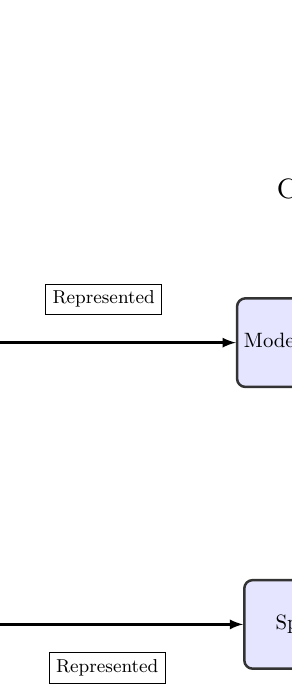
\begin{tikzpicture}[squarednode/.style={rectangle, 
					rounded corners, 
					very thick,
 					minimum width=3cm,
					minimum height=1.5cm,
					draw=black!80, 
					fill=red!10},
					squarednode2/.style={rectangle, 
					rounded corners, 
					very thick,
 					minimum width=3cm,
					minimum height=1.5cm,
					draw=black!80, 
					fill=blue!10}
					]
					
% To reduce all image, transform canvas
% forgets about image size, so 
% we need a bounding box
% This is lame, but works with Eduardo Thesis´s image (now black and white for elegance)

% don´t ask me about theses limits
% I just tried until I found which ones
%workded
\useasboundingbox (3,-4) rectangle (6,4);
\scope[transform canvas={scale=.75}]
         % Your actual drawing


%model nodes
\node[squarednode]  (concept) [anchor = west]{Conceptualization};
\node[squarednode2]  (mlang) [right of = concept, node distance=6cm, anchor=west] {Modeling Language};
\node[squarednode]  (model) [below of = concept, node distance=4cm, anchor=north] {Model};
\node[squarednode2]  (spec) [below of = mlang, node distance=4cm, anchor=north] {Specification};

% Arrows
\path[-latex, double, black, very thick] (concept.south) edge  coordinate[midway](c_to_m) (model.north);

\path[-latex, double, black, very thick] (mlang.south) edge  coordinate[midway](ml_to_s) (spec.north);

\path[-latex, double, black, very thick] (concept.east) edge  coordinate[midway](ml_to_c) (mlang.west);

\path[-latex, double, black, very thick] (model.east) edge  coordinate[midway](m_to_s) (spec.west);


\node [draw] (ml_to_cleg) [above of = ml_to_c, align=center, node distance=1cm, anchor=north]{\small Represented};

\node [draw] (m_to_sleg) [below of = m_to_s, align=center, node distance=1cm, anchor=south]{\small Represented};

\node [draw] (m_to_cleg) [left of = c_to_m, align=center, node distance=0.5cm, anchor=east]{\small Compose};

\node [draw] (ml_to_sleg) [right of = ml_to_s, align=center, node distance=0.5cm, anchor=west]{\small Compose};

\node (abs) [scale = 1.5, above of = concept, align=center, node distance=1.5cm, anchor=south]{\small Abstract};

\node (conc) [scale = 1.5, above of = mlang, align=center, node distance=1.5cm, anchor=south]{\small Concrete};

%\draw [dashed,<-,very thick](designerPathnew.north) |- (designerLegend.east);

    \endscope
\end{tikzpicture}
\caption{Modeling Diagram \citep{guizzardi_ontological_2005}}
\label{fig:model_diag}
\end{figure}

It is due noted the distinction made is between abstract and concrete ideas. The concrete are such because they have a material form which with one can interact. On the other hand the abstract concepts withhold the meaning conveyed by the concrete entities.

From the perspective of this work the model is the objective, so we center it on the interpretation of the diagram. That said, the model is an abstraction of a particular which resides in the world. So although it is the conceptualization that allows to compose a model, the target models need to have compatible conceptualization. An example, one cannot correctly create a model of soccer games using a conceptualization of the politics. This is called ``conceptualization appropriateness '' \cite{guizzardi_ontological_2005}.

The conceptualization comes with a modeling language to express its ideas. With this language it is possible to create a specification that represent a given model. But this specification must be in accord to the abstract model, otherwise it is no specification at all. 

Lastly should be noted that the relationships between the concepts are double-sided. Whilst a model is represented by a specification it is also interpreted from it. And while a conceptualization is used to compose a model, the model is a instance of that conceptualization.

Perhaps more important than these ideas is how they limit each other. And thus they need to be carefully accounted when modeling. This work thus abide to the conceptualization and modeling language provided by the Universal Foundational Ontology and OntoUML.
\section{UFO: a non-alien ontology} 

If the objective is to engineer a ontology there are many ways to take on this challenge. When the ontology to be engineered is of the domain or task type, a top-level, or more commonly named, foundational ontology is needed as basis for the new model. Altogether, an application ontology needs both a domain and a task ontology as a basis. How to address the creation of a top-level ontology is a complicated work and not on the scope of this text. It suffices to say that they are needed to build the other ontologies. In other words, domains and tasks are modeled using a foundational ontology and aplications are modeled combining a domain ontology and a task ontology.

Before delving deeper in UFO modeling specifications and concepts it is important to expose the perspective it uses to model the world. First is necessary to understand what are endurant and perdurant. Such concepts are introduced and studied in philosophy. They divide the being, or that which exists, in two possibilities, either it is a endurant or a perdurant. The former is a being that exists in time, it can be analyzed independently of the time. The latter is a beign which happens over time, and it needs that time-span to exists, thus is not independent of it. In a more simplistic manner one can say that perdurant are events and endurants are everything else. 

UFO or Universal Foundational Ontology created by \cite{guizzardi_ontological_2005}, is one of the most complete and used foundational ontologies in computer sciences. It leans on a heavy philosophical background and precise logical structure to provide a most complete modeling language. It is divided into different specifications UFO-a for endurants and UFO-b for perdurants. This work utilizes UFO-a because it is an ontology of an endurant and does not use UFO-b specifications. As such it is not thoroughly explained neither of them and this section focus on UFO-a only. whenever for simplicity whenever it is written UFO it is addressing UFO-a only.

\subsection{The Universal}

Central concept of the UFO is that of an \textit{universal}, it is the common proprieties found in different individuals. The concept is akin to a class or type in many of the modeling languages. It provides the common characteristics of a group of individuals. 

There are diverse types of universals which are classified according to how they deliver meaning to an individual. The first classification to be remarked is the distinction between sortal and dispersive. `` ... a Sortal Universal, which provides a \textit{principle of individuation} and \textit{identity} to the particulars it collects'' \citep{guizzardi_ontological_2005}. A dispersive universal embrace many concepts with different identities and thus do not convey a principle of individuation for its instances.

Rigidity of an universal provides another differentiation quality. ``A rigid universal is one that applies to its instances necessarily, i.e. in every possible world"\citep{guizzardi_ontological_2005}. For example, if there is a universal for \textit{Man} which specifies \textit{Person} in any possible world a given real person is identified by the person concept. While if it is a man it provides further identification, it is not a woman, and it remains a man in every possible world. An universal can also be \textit{non-rigid} which is the logical negation of rigid or \textit{anti-rigid} which is a more constraint form of non-rigid.

A universal which does not apply necessarily to at least one of its instances is non-rigid. \textit{Seatable} provides a nice example, suppose its instances are a given chair and a crate. The chair is necessarily seatable in every world whilst the crate can become unsteable and still be the same crate. Anti-rigid restricts that for every instance of the universal it must exist a world where it does not apply to that instance. Following the person example, a given man could be specified by the universal \textit{Child}, but it is only a child in his early years of life, in all other worlds he is no longer a child but a adult or elder.

Upon this classification \citeauthor{guizzardi_ontological_2005} brought together a typology for universals. This typology classifies and name the types of possible universals in UFO. This structure is depicted in \autoref{fig:Univ_diag}, and each of its leaves is a final classification for universals which are very important concepts for conceptual modeling. Those are defined and explained in the remainder of this section.

%Universal diagram
\begin{figure}[ht!]
\centering
\scalebox{0.65}{
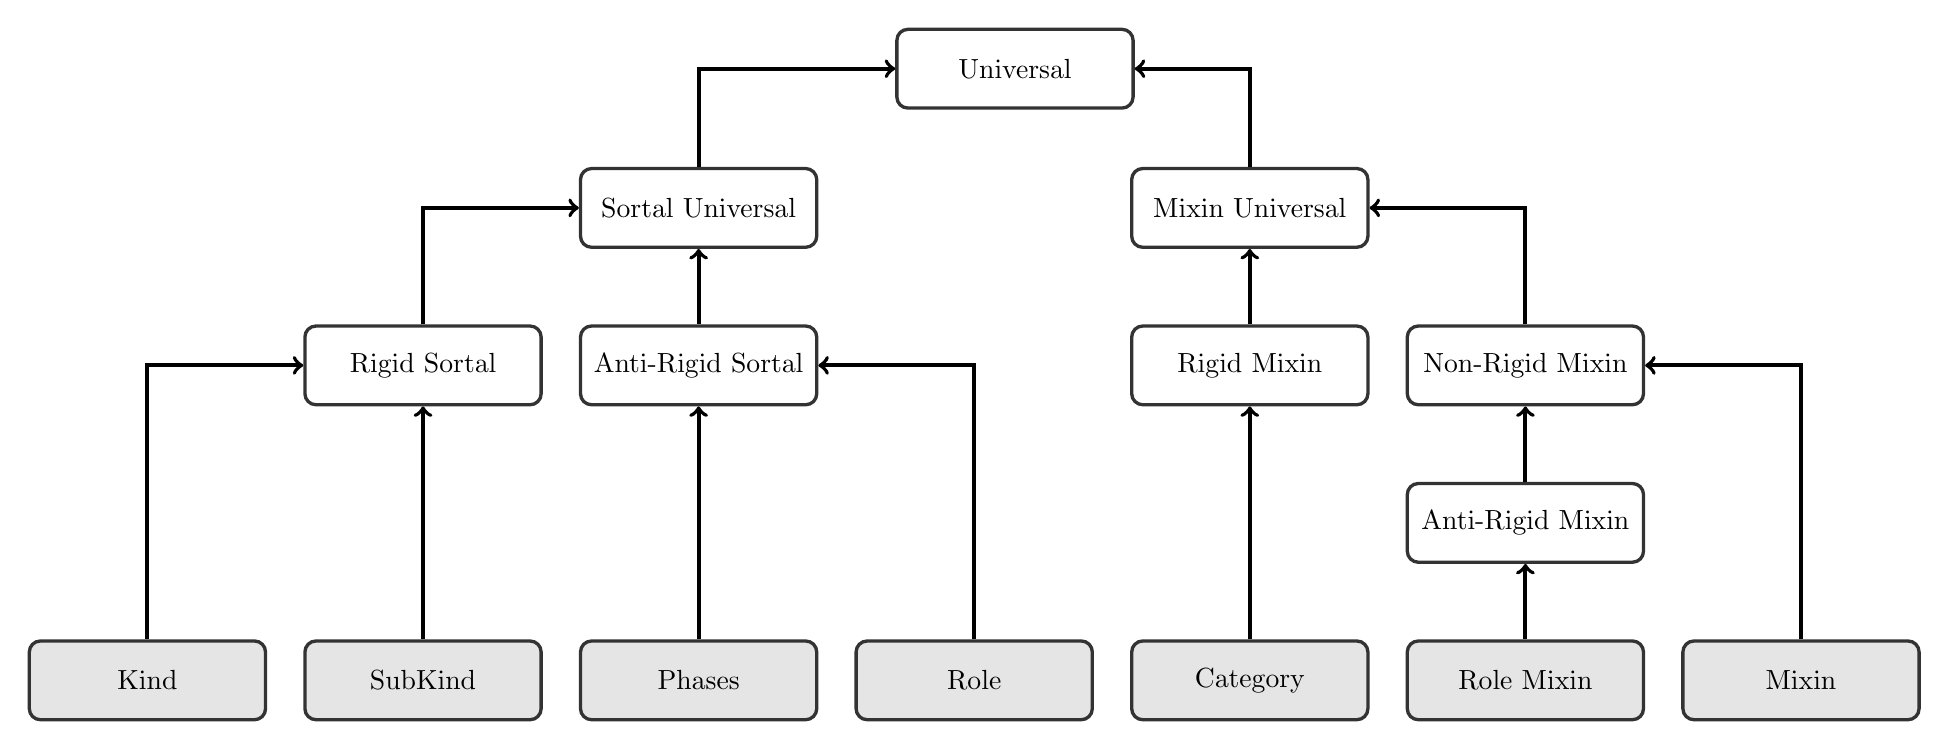
\begin{tikzpicture}[squarednode/.style={rectangle, 
					rounded corners, 
					very thick,
 					minimum width=3cm,
					minimum height=1cm,
					draw=black!80, 
					fill=white!10},
					squarednode2/.style={rectangle, 
					rounded corners, 
					very thick,
 					minimum width=3cm,
					minimum height=1cm,
					draw=black!80, 
					fill=black!10},
					node distance = 2.5cm
					]
					


%top node
\node[squarednode]  (Univ) {Universal};

%second level
\node[squarednode]  (Sortal) [below left of = Univ, xshift=-2.25cm] {Sortal Universal};
\node[squarednode]  (Mixin) [right of = Sortal, node distance = 7cm] {Mixin Universal};

% third level
\node[squarednode]  (ARigidSor) [below of = Sortal, node distance = 2cm] {Anti-Rigid Sortal};
\node[squarednode]  (RigidSor) [left of = ARigidSor, node distance = 3.5cm] {Rigid Sortal};

\node[squarednode]  (RigidMix) [below of = Mixin, node distance = 2cm] {Rigid Mixin};
\node[squarednode]  (NRigidMix) [right of = RigidMix, node distance = 3.5cm] {Non-Rigid Mixin};
\node[squarednode]  (ARigidMix) [below of = NRigidMix, node distance = 2cm] {Anti-Rigid Mixin};

% leaves
\node[squarednode2]  (SubKind) [below of = RigidSor, node distance = 4cm] {SubKind};
\node[squarednode2]  (Kind) [left of= SubKind, node distance = 3.5cm] {Kind};


\node[squarednode2]  (RoleMix) [below of = ARigidMix, node distance = 2cm] {Role Mixin};
\node[squarednode2]  (MixinL) [right of= RoleMix, node distance = 3.5cm] {Mixin};

\node[squarednode2]  (Cat) [below of = RigidMix, node distance = 4cm] {Category};

\node[squarednode2]  (Phases) [below of = ARigidSor, node distance = 4cm] {Phases};
\node[squarednode2]  (Role) [right of=Phases, node distance = 3.5cm] {Role};



% Arrows 
\draw [->, line width=0.5mm] (Sortal.north) |- (Univ.west);
\draw [->, line width=0.5mm] (Mixin.north) |- (Univ.east);

\draw [->, line width=0.5mm] (RigidSor.north) |- (Sortal.west);
\draw [->, line width=0.5mm] (ARigidSor.north) -- (Sortal.south);
\draw [->, line width=0.5mm] (NRigidMix.north) |- (Mixin.east);
\draw [->, line width=0.5mm] (RigidMix.north) -- (Mixin.south);
\draw [->, line width=0.5mm] (ARigidMix.north) -- (NRigidMix.south);

\draw [->, line width=0.5mm] (Kind.north) |- (RigidSor.west);
\draw [->, line width=0.5mm] (SubKind.north) -- (RigidSor.south);
\draw [->, line width=0.5mm] (Phases.north) -- (ARigidSor.south);
\draw [->, line width=0.5mm] (Role.north) |- (ARigidSor.east);
\draw [->, line width=0.5mm] (Cat.north) -- (RigidMix.south);
\draw [->, line width=0.5mm] (RoleMix.north) -- (ARigidMix.south);
\draw [->, line width=0.5mm] (MixinL.north) |- (NRigidMix.east);

\end{tikzpicture}
}%endscale
\caption{Universal classification Diagram \citep{guizzardi_ontological_2005}}
\label{fig:Univ_diag}
\end{figure}

Gray nodes at the bottom of the diagram are the types of universals present in UFO. Each contains the fundamental characteristics that define the concepts of the model. The arrows forms the specification path from which that type comes. Kind is a rigid sortal, which is a sortal universal that is a universal, and so on. Whatsoever each leave has its own meaning and definition that allows the modeler to stereotype each concept representing a universal.

`` << kind >> represents a \textit{substance sortal} that \textit{supplies} a principle of identity for its instances" \citep{guizzardi_ontological_2005}. The kind is then the representation of what is a rigid sortal, that is, in a given model all concepts which are rigid sortals are kinds. Subkinds are just specializations of kinds and can be omitted from a model without any lost. Any object in a UFO specification must be an instance of a kind, directly or indirectly.

Phases are a specification of kinds, and represent the different states of a kind has along the time of its existence. It is important that, when modeled, the phases of a kind constitute all of the phases it has in the world. That is, when modeling a person, and including his \textit{adult} and \textit{elder} phases, it would be incorrect without a \textit{child} phase. Phases then form a partition of a given kind existence.

Roles determine how a given entity plays a role in a certain context. Differently from phases, which depends solely on intrinsic proprieties, roles depends on external proprieties, that is, how the entity relates to the other entities. Roles, then, need to be connected by a relationship to a external  kind. Using the person example, the kind person can be related to roles such as \textit{student}, but it does need to have a relation, say \textit{enrollment}, with a \textit{school} kind. 

Mixin universals represents the dispersive concepts discussed before. Category is a collection of kinds, it is an abstract entity which unite common characteristics of the kinds it generalizes. Same is valid for Role Mixin, it is an abstraction of proprieties common to multiple Roles. 

The type defined as Mixin is basically everything else, it comprehends all non-rigid dispersive universals. Whatever fails to have the characteristics of the other types is a mixin. They represents proprieties which are essential to some instances but happens accidentally to the other ones. The best example to illustrate it is the seatable examples used previously, which it is essential to the chair but accidental to the crate.

Those classifications have a complete logical formal definition. Their description can be found in \cite{guizzardi_ontological_2005}.

\subsection{The wholes with parts}

Mereology is a very important component of ontologies. It is the theory which relates of the parts that compose a whole and how those parts relate to the whole. Simple as it may seem it is a very useful tool for accurately modeling complex wholes.

Defining parts and wholes in a very simple way may seem easy. Wholes are any concepts which has one or more parts and the concepts that together make up another one are parts. But this is not quite true for UFO, as it presents a \textit{principle of unity} in its mereology. For this principle to hold the parts of a whole need to be related between themselves, not only to the whole. Another diferentiation of this mereology is the existance of \textit{secondary characteristics of parts}. This defines the role a part play within the aggregate it belongs, i.e whether objects can share parts, or if an object can only exists if an specific part exists. 

Following is a further explanations of those important notions pertaining the theory of parts and wholes of UFO

\subsubsection{Principle of unity}

Prime reason for this principle is to deal with a conceptual problem very common in many mereologies. That using this theories purely can lead to very weird compositions which are not cognitively acceptable. Think of a set of parts and two wholes composed by these same set of parts. Most simple theories state that this wholes are identical, which is not necessarily true. It is easy to think of a band as a whole composed of its musicians but they can also be part of a group of friends or even a family. 

Integral wholes is the name given to a set of parts that have this principle. In other words, that have a unifying condition which bonds them in a specific way. Such connection should be not only a simple relation of any kind, it needs to tie the parts together in a way that changes their history. A good example is given by a molecule of a mass of water that is $H_2O$. While it is composed of H and O atoms if they didn't had a molecular bonding between them, the sharing of electrons, they wouldn't be a molecule of water.

\subsubsection{Secondary characteristics}

Parts convey a lot of meaning to its wholes, and the secondary characterization focus on explicitly understanding and classifying this meaning. There are two types of roles for parts, intimately related to how they behave in respect to the whole. If a part can be shared by multiple wholes, it is a characteristic named \textit{shareability}, or if it is separable from its whole, name it \textit{separability}.

Terming them secondary is done to emphasize that not all relations of this type has this propriety. That is, a part-hood relation might not feature such characteristics, but when they do, it express more meaning into the conceptual relation.

\subsubsection{Shareability}

Sheareability defines characteristics which address if a given part can be shared between different wholes. That is, if something can be a part of two different entities at the same time. With this it suffices to define a single type of part. 

The exclusive part, is a part-whole relation that states that its a part of its related individual or its a part of something else that is by itself a part of the related individual or the opposite, it is part of something of which the related individual is also a part. In other words if a given engine is a exclusive part of a car, it can be a part of the chassis which is part of that car, but never part of o museum which is not a whole with the car as a part. It might seem confusing but the exclusive is a good name, and its meaning is well applied in this concept.

This concept can be extended from individuals to universals creating the general exclusive part-whole relation. Is the same idea but relating universals instead of individuals, an universal A is a general exclusive part of an universal B, if every instance of A is exclusive part of some instance of B.

\subsubsection{Separability}

Understanding separability requires first to learn about ontological dependence. Existential dependence comes in a very intuitive way. If x is an individual existentially dependent of y, than necessarily y exists whenever x exists. Which can also be extended to universals creating the generic dependence. Individual z is generic dependant of the universal A, if whenever y exists a instance of A must exists.

Simply using the concept of dependence leads to a very intuitive secondary characteristic. Whenever there is a individual x and another one y, if y is existentially dependent of x and x is necessarily a part of y we say that x is an essential part of y. It is simply a part that without there is no whole, a good example is that one cannot have a living person without a brain, so brain is a essential part of living person. 

With this comes a notion of the extensional individual. It is the individual of which all of its parts are essential. That is, it needs all of its parts to exists, it cannot have some of them it needs all of them.

Using the other side of existentially dependence one can introduce the concept of inseparable part. This is a part which is existentially dependent of its whole. Important distinction comes from this notion, an essential part is not necessarily a inseparable part. When inseparable a part lifespan of existence is completely tied to the whole that contains it. Whilst the essential part can exists without the whole. I.e, a chassis is an essential part of a car, but the chassis exists a long time before the car does, while a brain is an inseparable part of a living person it existence is tied to the lifespan of the living person.

Lastly the concept of inseparable part can be generalized using the generic dependence of the part to a whole. We say that a mandatory whole is the individual instantiating an universal from which the part is generic dependent. An example is the heart of a living person, it can exist before a specific person, but it needs a person to exists. It can change the instance of person it is part of through a transplant, but some person is mandatory for its existence.

\subsection{Restrictions}

Restrictions are the name of some logical rules that binds the ontology. Their importance comes from expressing some imitating concepts from the world within the modeling language. In \cite{guizzardi_ontological_2005} does not address this feature in his theoretical basis. Nonetheless it is necessary for the development of ontologies and is included in OntoUML specification, where it is presented in OCL scripting. \citep{guizzardi_ontoUML_2004}

Logical sentences form those rules. They bind the cardinality of certain relations, the possibilities of generalization or even invalidate specific connections between some concepts. Restrictions like this have the purpose of impeding absurd representations of the modeled reality. In example, if in a model of persons we have an specification of man, an adult man, and it has a variable age. Without restrictions one could model an adult man with 10 years of age, which is an absurd. To correct this would be to add a restriction that for the adult man his age should be within 21 to 60 years.

Bureaucratic as they seem, restrictions are essential to model ontologies. They provide a means to express some limitations which can be hard to convey using the other ontological methods. Providing a way to introduce a logical reasoning inside the conceptual model, the rules, become a tool for the modeler to state how that reality works and behave. For the mater, in a given model it is possible to have a greater appropriateness using rules. That is, increasing the specificity of the model being able to be use abstraction about the reality intended.
\section{Emotions}
An important subject in the study of games is the emotions felt by the players. In MDA they feature as one of the three fundamental components of games. Emotions are traditionally a subject of psychology, but there are many studies focusing on emotions for games such as \cite{dillon_way_2010,bateman_implicit_2015,angelides_empirical_2014,karpouzis_emotion_2016}. This section covers baseline studies, on both games and psychology, meant to understand such complex subject and provide structure to this ontology.

There is no single line of research for emotions in psychology, however there are two major ways of studying them. One is called \textit{appraisal theory}, which consider emotions generated by appraisal and arousal, a valenced reaction to such appraisal \citep{ortony1990cognitive,scherer_appraisal_2001}. The other studies emotions as intrinsic manifestations, that is, there are a set of emotions understood as basic emotions which are natural to humans and independent of cultures and backgrounds, henceforth named \textit{basic emotion theory} \citep{ekman_are_basic_emotions_nodate,ekman_what_scientist_agree_2016}.

It is not in the scope of this work to discuss different psychological theories of emotions, or why and how they happen. What is of interest to this work is some structural model which exposes and classifies emotions that can be used as a basis for this ontology. That said, the appraisal theory models are more difficult to comprehend as they delve deeper in the terms of psychology and cognition. Whilst the basic emotion ones are simpler, much of this is due to the fact that appraisal theories are not about emotion words, that is, they do not intend to define emotion as they are used in common language. On the other hand, basic emotion theories study emotion from a perspective which focus on how the person interpret their own emotions and thus naturally it is defined in emotion words. 

The intention of this ontology is to be used by game designers and other persons interested in games, who do not necessarily have a deep knowledge of psychology. Basic emotions was then chosen as the theoretical foundation for the ontology of aesthetics because of its simplicity. The remainder of this section address two different models of basic emotions.

\subsection{Basic emotion models}

The following sections evaluates two different perspectives in basic emotion theory. One, built by \cite{dillon_way_2010}, is focused in the study of games, and therefore of great interesst to this work. The other one is a widely accepted and central theory created by \cite{ekman_are_basic_emotions_nodate}. Dillon's theory is not incompatible with Ekman's, actualy he uses the psychological theories of emotion created by many authors which agree with Ekman, and even use his theory. Thus this section analyzes two different takes on emotions studies, one purely psychological and the other applied to games, to find out how they can contribute to understanding emotions in games.

Also, it is important to make a clarification on basic emotions. This classification of an emotions in basic ones, is not in the sense that they are elements combined to create a more complex emotion, it denotes emotions which have a biological basis. The meaning behind this biological basis is that ``emotions are a product of our evolution" \cite{ekman_are_basic_emotions_nodate}. 

\subsection{The Atlas of Emotions}

Ekman created an atlas to illustrate his model which can be accessed at \url{http://atlasofemotions.org/} as of december 2018, it is the amalgamation of many years of research in emotions. This theory created by Ekman stands upon the assertion that emotions can be associated with physical reactions, to him, facial expressions.

The atlas identifies five basic emotions, anger, fear, disgust, sadness and enjoyment. Inside each basic emotion there are several emotional states, which are the ways a given person experiences this emotion. Each emotional state has its own intensity zone of the basic emotion it is related, this is illustrated by \autoref{fig:emotionalstates}. This zone represent how intense must be the emotion for the emotional state be manifested. Some of those states has zones that overlap, and can be felt at the same time. It is this conjunction of emotional states that represents the complexity of human emotion.

\begin{figure}[ht]
\hspace*{-1.25cm}
    \begin{tabular}{cc}
    
        \includegraphics[scale=0.5]{Images/AtlasEmotionalStatesGraphics/Figure_anger.png} & \includegraphics[scale=0.5]{Images/AtlasEmotionalStatesGraphics/Figure_Disgust.png} \\
        \includegraphics[scale=0.5]{Images/AtlasEmotionalStatesGraphics/Figure_Enjoyment.png} & \includegraphics[scale=0.5]{Images/AtlasEmotionalStatesGraphics/Figure_Fear.png} \\
        \multicolumn{2}{c}{\includegraphics[scale=0.5]{Images/AtlasEmotionalStatesGraphics/Figure_Sadness.png}}
    \end{tabular}
    
    \caption{Emotional States intensity}
    \label{fig:emotionalstates}
\end{figure}


Common responses in each emotional states are also identified in Ekman's model. They evaluate the usual reactions a person express when feeling a particular emotion state. There is also present the notion of mood, a mood is a mental state which causes a particular emotion to be more likely felt. 

\FloatBarrier
\subsection{The 6-11 model}

In his book \textit{On the way to fun} \citeauthor{dillon_way_2010} tackles the challenge of studying game design using emotions as his main perspective. His work consists of looking at successful games, that is, games which had a great acceptance of the public and received lots of positive criticism analyzing the emotions those games evoke. With this analysis Dillon creates a framework to understand how emotions behave in games, which is called 6-11.

6-11 stands as the name of the framework because this model is structured around 6 basic emotions and 11 instincts. The 6 emotions are fear, anger, pride, excitement, sadness and joy and the 11 instincts, survival, identification, collecting
, greed, aggressiveness, revenge, competition, protection/care, curiosity, communication, color appreciation are related as according to the framework diagram in \autoref{fig:611_diag}. The solid lines relates emotions to instincts they evoke and dashed lines instinct to the emotions they cause. Relations between emotions and between instincts appear in Dillon's book, but are not thoroughly explored by him. Most important are the relations between emotions and instincts. Thus for clarity of information relations between concepts of the same kind were left out of the diagram. 


%6-11 diagram
\begin{figure}[ht!]
\centering

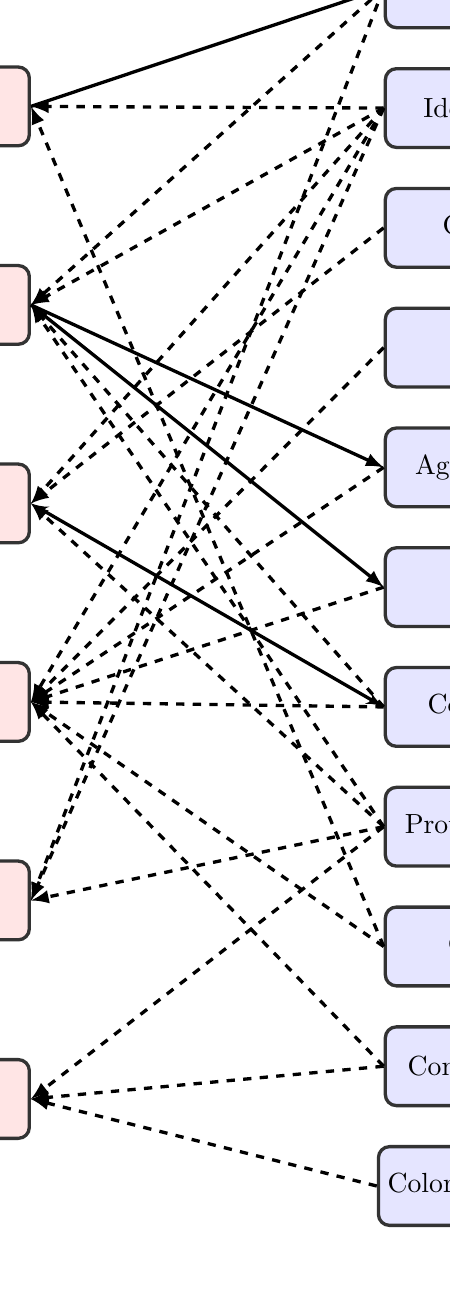
\begin{tikzpicture}[squarednode/.style={rectangle, 
					rounded corners, 
					very thick,
 					minimum width=3cm,
					minimum height=1cm,
					draw=black!80, 
					fill=red!10},
					squarednode2/.style={rectangle, 
					rounded corners, 
					very thick,
 					minimum width=3cm,
					minimum height=1cm,
					draw=black!80, 
					fill=blue!10}
					]
					
% To reduce all image, transform canvas
% forgets about image size, so 
% we need a bounding box
% This is lame, but works with Eduardo Thesis´s image (now black and white for elegance)

% don´t ask me about theses limits
% I just tried until I found which ones
%workded

\useasboundingbox (3,-8) rectangle (8,8);
\scope[transform canvas={scale=1}]
         % Your actual drawing


%emotion nodes
\node[squarednode]  (emo1) [anchor = west, yshift = 7cm ] {Fear};
\node[squarednode]  (emo2) [below of = emo1, node distance=2cm, anchor=north] {Anger};
\node[squarednode]  (emo3) [below of = emo2, node distance=2cm, anchor=north] {Pride};
\node[squarednode]  (emo4) [below of = emo3, node distance=2cm, anchor=north] {Excitement};
\node[squarednode]  (emo5) [below of = emo4, node distance=2cm, anchor=north] {Sadness};
\node[squarednode]  (emo6) [below of = emo5, node distance=2cm, anchor=north] {Joy};

% instinct nodes
\node[squarednode2]  (inst1) [right of = emo1, node distance = 6cm, anchor = west, yshift = 1.5cm]{Survival};
\node[squarednode2]  (inst2) [below of = inst1, node distance=1cm, anchor=north] {Identification};
\node[squarednode2]  (inst3) [below of = inst2, node distance=1cm, anchor=north] {Collecting};
\node[squarednode2]  (inst4) [below of = inst3, node distance=1cm, anchor=north] {Greed};
\node[squarednode2]  (inst5) [below of = inst4, node distance=1cm, anchor=north] {Aggressiveness};
\node[squarednode2]  (inst6) [below of = inst5, node distance=1cm, anchor=north] {Revenge};
\node[squarednode2]  (inst7) [below of = inst6, node distance=1cm, anchor=north] {Competition};
\node[squarednode2]  (inst8) [below of = inst7, node distance=1cm, anchor=north] {Protection/Care};
\node[squarednode2]  (inst9) [below of = inst8, node distance=1cm, anchor=north] {Curiosity};
\node[squarednode2]  (inst10) [below of = inst9, node distance=1cm, anchor=north] {Communication};
\node[squarednode2]  (inst11) [below of = inst10, node distance=1cm, anchor=north] {Color Appreciation};

% Arrows Emo to Inst
\path[-latex, black, very thick] (emo1.east) edge  coordinate[midway](c_to_m) (inst1.west);

\path[-latex, black, very thick] (emo2.east) edge  coordinate[midway](c_to_m) (inst5.west);

\path[-latex, black, very thick] (emo2.east) edge  coordinate[midway](c_to_m) (inst6.west);

\path[latex'-latex', black, very thick] (emo3.east) edge  coordinate[midway](c_to_m) (inst7.west);

%arrows Inst to Emo
%survival
\path[-latex, dashed, black, very thick] (inst1.west) edge  coordinate[midway](c_to_m) (emo2.east);
\path[-latex, dashed, black, very thick] (inst1.west) edge  coordinate[midway](c_to_m) (emo5.east);
%Identification
\path[-latex, dashed, black, very thick] (inst2.west) edge  coordinate[midway](c_to_m) (emo1.east);
\path[-latex, dashed, black, very thick] (inst2.west) edge  coordinate[midway](c_to_m) (emo2.east);
\path[-latex, dashed, black, very thick] (inst2.west) edge  coordinate[midway](c_to_m) (emo3.east);
\path[-latex, dashed, black, very thick] (inst2.west) edge  coordinate[midway](c_to_m) (emo4.east);
\path[-latex, dashed, black, very thick] (inst2.west) edge  coordinate[midway](c_to_m) (emo5.east);
%Collecting
\path[-latex, dashed, black, very thick] (inst3.west) edge  coordinate[midway](c_to_m) (emo3.east);
%Greed
\path[-latex, dashed, black, very thick] (inst4.west) edge  coordinate[midway](c_to_m) (emo4.east);
%agressivenes
\path[-latex, dashed, black, very thick] (inst5.west) edge  coordinate[midway](c_to_m) (emo4.east);
%revenge
\path[-latex, dashed, black, very thick] (inst6.west) edge  coordinate[midway](c_to_m) (emo4.east);
% Competition
\path[-latex, dashed, black, very thick] (inst7.west) edge  coordinate[midway](c_to_m) (emo4.east);
\path[-latex, dashed, black, very thick] (inst7.west) edge  coordinate[midway](c_to_m) (emo2.east);
%Protection/care
\path[-latex, dashed, black, very thick] (inst8.west) edge  coordinate[midway](c_to_m) (emo2.east);
\path[-latex, dashed, black, very thick] (inst8.west) edge  coordinate[midway](c_to_m) (emo3.east);
\path[-latex, dashed, black, very thick] (inst8.west) edge  coordinate[midway](c_to_m) (emo5.east);
\path[-latex, dashed, black, very thick] (inst8.west) edge  coordinate[midway](c_to_m) (emo6.east);
%curiosity
\path[-latex, dashed, black, very thick] (inst9.west) edge  coordinate[midway](c_to_m) (emo1.east);
\path[-latex, dashed, black, very thick] (inst9.west) edge  coordinate[midway](c_to_m) (emo4.east);
%communication
\path[-latex, dashed, black, very thick] (inst10.west) edge  coordinate[midway](c_to_m) (emo4.east);
\path[-latex, dashed, black, very thick] (inst10.west) edge  coordinate[midway](c_to_m) (emo6.east);
%color apreciation
\path[-latex, dashed, black, very thick] (inst11.west) edge  coordinate[midway](c_to_m) (emo6.east);


    \endscope
\end{tikzpicture}
\caption{6-11 model Diagram}
\label{fig:611_diag}
\end{figure}

Differently from the Atlas of emotions, Dillon's identifies 6 basic emotions. Some of them very akin o those of the atlas while others even feature in the atlas as emotional states. That said, the emotions section of the 6-11 framework is very similar to the emotions proposed by Ekman and there is no novelty remark to be made.

Instincts are introduced by this model. Dillon does not give a precise definition of instincts as ``the analysis of instincts can spur disagreement among sociologists and psychologists''\citep{dillon_way_2010}. Instead he provides some common accepted characteristics of instincts:
\begin{itemize}
    \item Are automatic
    \item Are irresistible
    \item Occur at some point in development
    \item Are triggered by some event in the environment
    \item Occur in every member of the species
    \item Cannot be modified
    \item Govern a behavior for which the organism needs no 
training
\end{itemize}

Upon this he states that for this model's purpose the focus lies upon the fact that instincts are triggered by some event in the environment and that ``we can simply take the others for granted and let sociologists debate over them.''\citep{dillon_way_2010}. Which means that the framework models not what or why such instincts are present in games, but how they happen.

The last part of the 6-11 framework is how each emotion relates to each instinct. This is a causal relation, when a given emotion evokes a certain instinct or a instinct triggers a particular emotion. The purpose of this relation is to be possible to analyze how those two concepts interacts within a game. How a given emotion is felt by the player and what is responsible for this feeling, and which consequences this emotion brings to him. 


	\chapter{Crafting an Ontology}

This chapter covers how a domain ontology about boardgames was built. The ontology, henceforth called OntoBG, is composed of 3 blocks and constructed upon the theoretical framework of the Universal Foundational Ontology or UFO \citep{guizzardi_ontological_2005}, using the OntoUML modeling language as described in \cite{guizzardi_ontological_2005,guizzardi_ontoUML_2004,guizzardi2015towards}. 

The purpose of separating the ontology into three sub-ontologies is to put together the three ontologies of mechanics, dynamics and aesthetics in a coherent and understandable single ontology, this will expose the structure of the MDA framework used as theoretical principle of this thesis. Each of those sub-ontologies is assembled using a specific methodology. The particulars of their creation will be further explained in the following sections.

For clarity purposes, these three sub-ontologies of the ontology are named OntoBG-M, OntoBG-D and OntoBG-A, respectively for the mechanics, dynamics and aesthetics.

Before introducing the specifics for each sub-ontology of the OntoBG it is important to specify how it can be used to model this particular domain. Due to the broad philosophical foundation of UFO, this subject will be split in two sections. The first addressing this philosophical theory and the general concepts in this model, afterwards it is addressed how it will be applied in the domain of boardgames to give fruition to OntoBG.


\section{Thinking of UFO} 


Games are endurants as far as this ontology is concerned. So UFO-a is used in this work to model such endurant. The interest, then, is to look up to its characteristics as an endurant not a perdurant. There is some aspects of games that can be seen as perdurants, a specific match, the social interaction of games and other ones. But for the MDA framework games are studied as endurants, static things that exist.

First and foremost, an ontology is founded upon concepts of a given domain. To build it we need to acknowledge and understand the reality to be conceptualized. In this case, the more abstract concepts comes from the MDA framework definitions: games are mechanics, dynamics and aesthetics. For the specifics, each will have a different approach, as they are very different in nature. For mechanics it was possible to build the reality to be modeled perusing many authors on game studies as well as widely accepted knowledge bases of board games. Dynamics proved a more difficult subject, it was needed to use research methods to uproot the reality, as there are little specific literature in the area. Emotion models were studied to bring about the aesthetics reality and become a basis for this work's ontology.

Reality provided through the MDA definition of each part implies that mechanics, dynamics and aesthetics are all kinds. Clearly they are sortals, given they provide identity to all parts of the game. Rigidity comes from the necessity of games to have those parts. MDA understands that games are composed of three components, and they are necessary to all games, they define the game. With a big number of kinds in the ontology, for simplicity all are stereotyped as kinds and never as subkinds.

Featuring a big number of concepts, if OntoBG had all possible relationships among those concepts it would become useless, as nobody could understand it. With this in mind, many of such relationships are omitted. But the ones that are in the ontology will be examples of how to express an information in the ontology. Should then be seen as templates to be extended to any other concepts it seems to fit. To help this simplification, the logical restrictions of the model will express how to relate two concepts. More specifically how one cannot relate two individuals or about the correct cardinality for some relationships. 

\subsection{OntoUML}


OntoUML is a language created to express the ontologies created using UFO. His specification are perfectly matched to UFO-a definitions and concepts, which means it is a language to model endurants. It is made similar to UML, hence the name, because of the proximity of UFO and UML standards. Many concepts well established in UML are in accord with UFO, only needing some specifications to be correct. Thus OntoUML is a heavyweight extension to UML to allow UFO standards to be written in UML. 

To make use of this language, this work uses Menthor, a free application developed by \citeauthor{guizzardi_ontological_2005}. Menthor was created through the specifications of OntoUML, it uses these standards to be a tool for creating domain ontologies from UFO. Similarity to UML makes it familiar and easy to use. Restrictions are scripted in OCL. Overall, it is a powerful yet simple tool to create ontologies. Thus its appropriateness for this work is undeniable.

Used to provide visual representation of the model, OntoUML is of great use to understand the data representation and modeling. Thus it is used mainly as a way to convey the structure of OntoBG keeping it understandable and readable.
\section{How to model board games} 

The perspective of modeling board games in accord with UFO is not unique neither simple. As with any modeling activity, there are many possible interpretations of the concepts of the domain, which means that a focus is needed. This focus is to make the choices of interpretations giving more importance to certain aspects of the concepts, with some specific goal in mind. As example, one could model board games as a social activity, focusing on player interactions and consequences of play, another perspective is to model the physical artifact, focusing on the materials and forms used in board game elements.

This ontology focus its lenses in a MDA model perspective, that is, it looks to board games as composition of 3 concepts. That gives a broader spectrum for the perspective of OntoBG, which means it comprehends the artifact, the play of the game as well as the consequences of play. But most important is that MDA looks into games as a construct, that is, it focuses on the fact that it is made with intention, during the games' design. Even when looking on the play of the game or the aftereffects of it, it does so considering them as part of the constructed entity. That said, is important to note that all the modeling choices done in this work take this perspective into account to be faithful to the MDA basis. 



Addressing the modeling directives used to create this ontology is important to be sure that all the choices are reasonable with each other. This should clearly state the view of the world represented by this model. OntoBG uses the following directives for modeling board games:

\begin{itemize}
    \item Mechanics, dynamics and aesthetics are viewed as kinds, as well as mandatory parts of board games
    \item Concepts to be included need to be present on a given board game, that is, concepts exclusive of digital games are not included.
    \item Relationships between mechanics and dynamics or dynamics and aesthetics maintain the same meaning as the MDA framework
    \item Concepts that are neither a mechanic, dynamic or aesthetic cannot feature in the ontology
\end{itemize}

OntoBG will be created as a lightweight ontology. That means it does not provide an axiomatization of the domain. Not being strict on concepts definitions is essential when creating such a preliminary work. Especially when addressing a domain such as games, which are defined through common knowledge rather than scientifically. This also increases the possibility for contribution on expanding the ontology as any one with experience can provide valuable ideas. Not being comprehensive, this work' ontology needs to be enhanced through peer contributions to cover more thoroughly the board game domain.


\section{Mechanics}
The mechanics ontology will be a restructuring of the board game mechanics ontology created previously in \cite{kritz_buildingOntology}. Although it was created using a different methodology it will be used as a foundation for this mechanics ontology. There is a necessity to adapt this ontology and its description to fit in the UFO standards. It will not change much of the structure of the ontology and the main idea will remain untouched. But this will enrich naturally the ontology as the UFO provides a much larger semantic value than the previously used methodology.

To access the situation all of the nodes in the original ontology will be translated as kinds and subkinds. The is-a relations between the nodes will become generalizations as in the OntoUML specifications they are semantically equal.
\section{Dynamics}

Dynamics might be the most complicated domain to model in this ontology. Using the definition provided by the MDA framework dynamics become almost about everything. In an essay \cite{leblanc2006tools}, one of the creators of MDA, states ``When we view a game in terms of its dynamics, we are asking, 'What happens when the game is played?'' and the complete answer to this question when we are looking into the whole domain of board games becomes overwhelming as there is a multitude of things happening during a single gameplay, there is even more about all possible plays of all possible games. 

Another difficulty found is the lack of specific research on dynamics of games. Although many authors acknowledge and speak of dynamics they do so when focusing their efforts in other aspects of games. So they do not convey a definition of the term neither a good pool of examples. With this there is nowhere to find a big set of terms and concepts with a structure in dynamics of games like it was done with mechanics and aesthetics.

To workaround this troublesome situation this work brings about a quantitative and qualitative research to provide an initial knowledge of dynamics of board games. This is done by using a focus group composed of game designers to evaluate on names and concepts of dynamics. Following with a survey applied more widely to validate the results of the focus group and provide more suggestions. The resulting set of concepts will be then evaluated through the survey results and pruned when needed, after such filtering they will be used to compose the ontology of dynamics.

\subsection{The focus group}

A focus group is a method to generate data based on individual experience and the discussion of such individuals on those experiences. Those individuals should have common expertise in the topic to be addressed in the experiment. Even better is if the participants have a good amount of knowledge and experience on the subject. According to \cite{jenny_methodologyfocusgroup_1994} the most important data of a focus group is provided by the interaction and discussion of the individuals. Nonetheless a focus group have to remain focused on the topic to be addressed and thus need to be directed correctly to provide better quality data for the reasearch. \citep{liamputtong_focusgroup_2011,rabiee_focus-group_2004,jenny_methodologyfocusgroup_1994}

The selection of individuals for this focus group should, of course, be composed of the target users of this methodology, designers of board games. Also it intends to collect data on dynamics, which happens during the play of the game. Thus long time players of board games should also be able to provide valuable insight, and are included in this selection. 

Designers and play-testers of the \textit{Casa do Goblin} collective agreed to be our focus group and will endeavour in this activity. They all have experience in the board game domain and have interest in OntoBG as a creation or analysis tool. The participating designers were also both new and experienced ones. The ten participants were composed of 5 men and 5 women, from 23 to 40 years old.

Although experts in board games, the participants have differing notions of dynamics or no understanding at all of the specifics. As such it is needed to thoroughly explain the dynamics concept of the MDA to them. Then designers participants will brainstorm on names or terms of dynamics they believe pertain to board games. Afterwards they will discuss what was proposed on the brainstorm to filter unfitting concepts and to further develop the ones that require extra atention.

\textit{Casa do Goblin}'s participants will be introduced to the dynamics concept using the definition in the MDA model, as well as further explaining of the notion according to this works's fundamentals. To clearly illustrate the concept, the example of \textit{movement} - \textit{run} - \textit{fear}  is used. Also they will be encouraged to compose generic and simple examples like this one to be sure they grasped the meaning. 

The discussion will be directed towards generating words for dynamics, that is, to explicate concepts they believe to be dynamics into simple words. To provide an anchor from where to start the mechanics featured in this OntoBG-M will be fixed on a board in everyone' views. The purpose of the mechanics will be to be used as basis for thinking of dynamics they found in games, that is, looking to the mechanics and thinking which dynamics emerge from each of them.

Provided the initial basis of words and concepts the group then will review the words generated and discuss what they mean, how they present themselves in games and wetter it is or not a dynamic. If needed little adjustments should be made and the words will become concepts to be used in OntoBG-D, that is, become names of dynamics.

Discussion made during the whole process will be acknowledged as possible concepts and relations that are not dynamics names. In example abstract concepts used to structure the dynamics, connections between types of dynamics, maybe even part-whole relations.



\subsection{Survey on dynamics}

At the begining of the survey there will be a short explanation of what is a dynamic of board game according to the MDA. This is to be sure all subjects are on the same terms to the concepts. Also for statistical purposes and further analysis there are questions about their relation to the board game world (designer, producer, hobbyist) and how long have they known and played board games. This distinction comes from the proposal of MDA that the player of the game and the designer have different perspectives of the game. Which can lead to a significant difference in their opinions about dynamics.

The survey will be composed of questions based on the results of the focus group. For each term created the survey will have a 5 point traditional likert scaled questions. Surveyed subjects answer how much they agree or not with the term as a dynamic that actually happens in games. One of its advantages was having the neutral option between agreement or disagreement, what would allow for answers like not knowing or not understanding. For verification purposes, before the actual questions are made the survey requires some information about who is filling it. These questions inform of how the subject is related to board games and how frequently he plays board games. \citep{devellis2016scale}

To establish the concepts that would feature in the survey a trimming was necessary. Fifty seven concepts, resulting in 57 questions, would lead to a large survey. Large surveys with obligatory questions are less likely to receive answers which could lead to insufficient number of answers. To adjust this the 57 concepts obtained from the focus group will be narrowed. The redundant concepts, which are contained in one another, will be removed. Keeping only the more generic ones. Also, similar concepts which can together be abstracted into a new one that does not feature in the list will be removed as well. Favoring the more general concept. \citep{malhotra2012pesquisaMarketing}

Furthermore if the subject wanted it could suggests new dynamics he felt were missing. And also provide an e-mail address to be further informed about this research if he was interested. 

The actual survey submitted to the public can be found in \autoref{appendix:a1} the Portuguese version and in \autoref{appendix:a2} the English version. It was made and submitted in both languages to achieve a greater number of answers which leads to greater diversity of opinions. The survey was created unsing google forms and conveyed through facebook and whatsapp groups with board game interests as well as in the board gameGeek forum. The results will be considered closed after a week of being released.

The results collected are expressed and analyzed in chapter 4. There will be some statistical testing on the data. The intent is to decide the best way of using it, whether simply merging the answers from all groups or putting different weights in each. This will be decided through an ANOVA test, which will determine if the data from different groups have any significant discrepancy. If none is found, all answers will be considered equally, in the other case the professionals should be considered to be better quality data, thus given a bigger weight. After this decision the final value for each concept will be evaluated.

Finally, the concepts that will be used to create OntoBG-D will be the ones with a value greater than 3. Those are the concepts which majorly had answers agreeing with them.

\subsection{Developing the ontology}

After acquiring and processing the data it will be used as a baseline for the concepts of the OntoBG-D. Grouping them together, by similarity, or by generalization characteristics. This ontology will bring up a starting notion of how to address dynamics in board games. As any part of this ontology it does not intend on being comprehensive or complete. It does then provide some insight on different ways to understand the dynamics collect. That is, the final classification and relations present in the ontology should be viewed as suggestions.

Correlating and classifying the concepts featuring in the OntoBG-D will be done in accordance to the author experience as well as the discussions made during the focal group. Remaining truthful to the idea of comprising the ontology with experience, making it tune in with the designers needs.
\section{Aesthetics}

The aesthetics ontology domain is centered on emotions, as such this ontology is created with foundation in emotions theories. In this light this ontology is based in two theories, the \cite{dillon_way_2010} 6-11 model, which is a theory of emotions in games, and the one presented in \cite{ekmans_atlas} Atlas of Emotions. This last theory was built in a psychological view with no direct relation to games. The objective of using both theories in union is to benefit from the detailed perspective of Ekman's approach, which brings a rich understanding of how emotions behave, while using Dillon's simpler approach to appropriately connect the whole theory into the games domain.

Fusing both theories is not inconceivable because both precepts the existence of basic emotions. Their understanding of basic emotions although slightly different have a lot of overlaps and are totally compatible. That said, Ekman's model is adopted for the emotions, as it is far more detailed and complete, in detriment of the 6-11 model. From Dillon's model we harness the instincts section, it provides insight in how emotions behave in games. 

Established those directives, the particular method for modeling emotions and instincts is broadly described in the following subsections.

\subsection{The modeling of emotions}

OntoBG-A is centered around the five basic emotions found in the Atlas of Emotions. The goal of OntoBG is to express boardgames in a way that designers can expand their knowledge about their games. As such this ontology features the emotions states of the atlas as subkinds of the basic emotions. This is due to some advantages these concepts introduce in the ontology. First when analyzing games, the broadness of the emotions can create confusion or ambiguity whilst using emotional states specificity provides more clarity in how the game affects the player. It is due to this specificity of the states that when relating to instincts the user of the model can pinpoint more precisely how that instinct interacts with the game. Also emotional states not being exhaustive abides to one of the goals of OntoBG, which is to be expansible according to the needs of the designer. Opposing the emotions that are static for the theory, thus using only them the model would become static as well. With this the designer can include new emotional states he identifies in his game giving him the tool he needs to understand the emotions behaviour in his game.

Composite emotions are acknowledged in the Atlas of Emotions as it is possible for a given person to feel different emotions simultaneously \citep{ekman_are_basic_emotions_nodate}. When this event occurs the union of emotions provokes different reactions and thus it is useful to include such concept in OntoBG-A. But Ekman's model does not explicate any composite emotion thus the inclusion of this concept in this model come as a category with no kind as an example. With this the user of the model that needs to analyze a particular composite emotion can introduce it as a specification of this category and identify which emotions compose it by parthood relationships.

Instincts feature as kinds connected to the emotions according to \citeauthor{dillon_way_2010}, using the needed adaptations of disposed emotions. Relationships from instincts to emotions should not be viewed as unique and static, as relating instincts to emotional states is also possible and encouraged. But for simplicity we stick to the theoretical framework used as basis.
\section{Using the ontology}

The main objective of OntoBG is to help designing and analyzing games. To achieve this it was created a Prolog program implementing the data model, containing the rules for describing games using the OntoBG specification, thus allowing a user to have a database of games. From such database one can extract information he needs from the ontology using the rules in the program.

Prolog was chosen as it is a logical language that is widely used and have great support. Logic is used to express the rules of the ontology. Rules that provide a reasoning which match the knowledge contained in OntoBG. In other words, the rules explain the inherent data of the ontology in system. This system is then used to actual manipulation on the ontology and associated database. 

Querying the base of games can be made using the Prolog commands. Those will bring some information required. Such as, if a game is already in the database, if there is a similar game or even to suggest a variation of a game. By manipulating the data modeled through this program, the user can find useful information to his work. 


\section{Scope delimitation} 

Important reminder is that OntoBG is not comprehensive and do not claims to become so. To map all possible ramifications of games might be impossible. So this ontology shall be seen as a preliminary work towards understanding and modeling the nature of board games. This scope delimitation is not about removing, it is about gaining. With this, OntoBG can be flexible to attain the most simple needs of a researcher or designer while still being able to grow more complex. Reducing it also turns it more palatable for anyone, not familiar with modeling or ontologies in general, to use.

Fixing the scope on board games is important to lean this work. This is important to achieve the objectives of OntoBG. It permits that the ontology can be increased with ease and simplicity. Also bringing consistency to the knowledge it represents, guaranteeing that OntoBG is easy to understand and use.



	\chapter{Dynamics: experiment results and analysis}

This chapter comments and exposes the data obtained in the experiment of dynamics. After explicating the contents of the results it uses a statistical method to evaluate the data and decide how to use it. Lastly it makes some worthy appointments noted throughout the experiment, which might be of great use in expanding it in the future.

\section{Focus group} 

Results from the focus group came in form of knowledge on board game dynamics. This knowledge was represented in form of 57 ideas which were proposed and discussed by the group. Analyzing the collected ideas and comprising them into a more compact list was done shortly after, which was important to do before this ideas could be used in the subsequent tasks. 

Primarily the group proposed ideas of dynamics. It developed a lot of concepts, which were then discussed and checked whether they were dynamics or not. Many concepts were mentioned by more than one person even if in different terms. This means the group was well aligned in how they understand the dynamics. Other concepts met a big dissension on whether they were dynamics or not. Further studies should be made to evaluate this, thus they were excluded from this work. The group could not associate some ideas, which seemed dynamics, with a proper mechanic. Without such connection they were not included in this ontology. Discussing the concepts proved to be most valuable. Some of them did not appeared to be dynamics in a first glance. But in another perspective or situation they were dynamics.

Apart from the dynamic concepts created the discussion featured their relation to mechanics and aesthetics. As a group, they related many dynamics to the other concepts when explaining them or trying to understand. Also sometimes relating dynamics to each other. Establishing that some are incompatible with each other, as well as generalizations between them.

Finally a list of 40 dynamics was comprised. They can be found in the following list.Those were used to form the questions of the survey. 
\begin{multicols}{2}
\begin{itemize}
    \item 1 - Do an action to reduce other players options
    \item 2 - Collateral effect: do A resulting in B intending C.
    \item 3 - Use an action to discover information, see other players reaction.
    \item 4 - Block another player
    \item 5 - Use an action to force a change in the game state (phase, turn, etc)
    \item 6 - One versus all, one player decides to attack all others
    \item 7 - All versus one, players uniting against one
    \item 8 - Ally with another player
    \item 9 - Pursue another player
    \item 10 - Survive, play to evade elimination
    \item 11 - Chain automatic effects (combo)
    \item 12 - Reduce or render useless a resource
    \item 13 - Defend from a player using another one
    \item 14 - Parallax: Change a point of view to create a better result for himself
    \item 15 - Avoid to acquire points to get some other benefit (playing early next round)
    \item 16 - Camping, in a position or determinate action
    \item 17 - Stop the progress of the game, delay the endgame
    \item 18 - Play accounting to your next actions, plan a series of actions.
    \item 19 - Alpha player: Player that forces the others to play as he wants
    \item 20 - Protect an specific position or pieces
    \item 21 - Play safely, do not take on risks only play on certainty
    \item 22 - Rituality: Repeat the same way of playing looking for the same results as before
    \item 23 - Counting cards, tokens and other resources
    \item 24 - Play riskily, pursue greater risks for greater gain
    \item 25 - Pursue self defined objective instead of the game objective
    \item 26 - Accelerate the end of the game
    \item 27 - Do a sacrifice for greater gains
    \item 28 - Distraction: Use an action to change other players attention from your real intention or objective
    \item 29 - Change strategy because of the game state
    \item 30 - Deduce hidden information through open information
    \item 31 - Communicate with allies indirectly so other players does not notice
    \item 32 - Forfeit the game
    \item 33 - Cheating: break the game rules
    \item 34 - Trolling: play to annoy other player rather than win the game
    \item 35 - Intimidate: use a stronger position to force another player to play as you want
    \item 36 - Bluffing: relay false information to manipulate other players actions
    \item 37 - Convince the other players
    \item 38 - Confound a player to induce a bad play
    \item 39 - Excluding another player
    \item 40 - Small talk: talking all the time to distract other players
 \end{itemize}
\end{multicols}

\subsection{Cruious cases}

Some concepts which arose during the focus groups discussions were very interesting although they did not reached the final list. This was because they were very complicated cases. But the fact that they were brought to discussion, is by itself a great contribution. 

One was Chaos, meaning a condition of disorder in the
game, that is, chaos made by the players. It was very
surprising to most, and through discussion they couldn’t
agree whether it is or not a dynamic. The most interesting
factor on this discussion, however, is that if it is a dynamic,
other possible conditions, like funny, tense and ordered,
would also be dynamics. On the other hand, it is also
possible that those concepts are actually part of Aesthetics,
as defined in the MDA\cite{Hunicke2004} since they could be associated to
emotional states.

Another case is the change of rules during the game.
This situation can happen in gameplay in some situations,
more notably when players notice a confusion or wrong
interpretation of the rules. It could also happen when players
find something broken while creating games, and it is
common on children’s play. The first case always rise the
question “does we keep playing wrong to avoid changing
the game as it is now, or from now on we play correctly?”.
Hence the possibility of being a dynamic, since it comes
from the decisions the players make. However, since it is
not part of the gameplay itself, it can be considered a meta-game
event.

The focus group also detected another common situation
in board games that can be considered a meta-game action:
a player needing or wanting to undo his last move or play,
including the case that it was impossible to be made with
the correct rules. 

All of those situations are left unanswered in this work.
They push way through the boundaries of our scope of
preliminary work, requiring more study and thought, and
were left for future development.


\section{Survey data}

Answers to the survey were collected for one week time, from 12/13/2018 to 12/20/2018. Featuring a total of 196 answers, which were divided in two groups consumers with 174 reply's and industry totalling 22 answers. Then the average value for each question in each group was computed. Those values are represented in \autoref{tab:SurveyIndustry} and \autoref{tab:Surveyconsumer}. The number of the question is the order in which it appears in the survey.

\begin{figure}[h]
\begin{adjustwidth}{-1.5cm}{}
    \centering
    \pgfplotstableread{
Question    Average
1   4,23
2   3,82
3   4,36
4	4,32
5	4,50
6	3,50
7	3,68
8	3,73
9	2,55
10	3,50
11	3,86
12	3,64
13	3,18

}\mytable

\pgfplotstabletranspose[string type,
    colnames from=Question,
    input colnames to=Question]\mynewtable{\mytable}
    
\pgfplotstabletypeset[string type]{\mynewtable}
\newline
\vspace*{0.01 cm}
\newline
    \pgfplotstableread{
Question    Average

14	4,05
15	4,00
16	3,27
17	2,55
18	4,55
19	2,86
20	4,00
21	3,45
22	3,09
23	3,68
24	3,32
25	4,00
26	4,32
27	4,45

}\mytable

\pgfplotstabletranspose[string type,
    colnames from=Question,
    input colnames to=Question]\mynewtable{\mytable}
    
\pgfplotstabletypeset[string type]{\mynewtable}
\newline
\vspace*{0.01 cm}
\newline
    \pgfplotstableread{
Question    Average

28	4,41
29	4,14
30	3,14
31	2,18
32	2,09
33	2,50
34	3,14
35	4,00
36	3,82
37	3,00
38	2,18
39	2,27
40	3,77
}\mytable

\pgfplotstabletranspose[string type,
    colnames from=Question,
    input colnames to=Question]\mynewtable{\mytable}
    
\pgfplotstabletypeset[string type]{\mynewtable}

    \caption{Survey averages for industry}
    \label{tab:SurveyIndustry}
\end{adjustwidth}
\end{figure}
\begin{figure}[h]
\begin{adjustwidth}{-1.5cm}{}
    \centering
    \pgfplotstableread{
Question    Average
1	4,07
2	3,90
3	3,92
4	4,16
5	4,04
6	3,21
7	3,35
8	3,72
9	2,62
10	3,48
11	4,16
12	3,41
13	3,17

}\mytable

\pgfplotstabletranspose[string type,
    colnames from=Question,
    input colnames to=Question]\mynewtable{\mytable}
    
\pgfplotstabletypeset[string type]{\mynewtable}
\newline
\vspace*{0.01 cm}
\newline
    \pgfplotstableread{
Question    Average

14	3,57
15	3,75
16	3,01
17	2,94
18	4,44
19	2,68
20	3,93
21	3,46
22	2,88
23	3,75
24	3,07
25	3,78
26	4,06
27	4,11

}\mytable

\pgfplotstabletranspose[string type,
    colnames from=Question,
    input colnames to=Question]\mynewtable{\mytable}
    
\pgfplotstabletypeset[string type]{\mynewtable}
\newline
\vspace*{0.01 cm}
\newline
    \pgfplotstableread{
Question    Average

28	4,34
29	4,06
30	2,63
31	1,88
32	1,76
33	2,27
34	3,06
35	3,71
36	3,82
37	2,93
38	2,07
39	2,26
40	3,91
}\mytable

\pgfplotstabletranspose[string type,
    colnames from=Question,
    input colnames to=Question]\mynewtable{\mytable}
    
\pgfplotstabletypeset[string type]{\mynewtable}

    \caption{Survey averages for consumers}
    \label{tab:Surveyconsumer}
\end{adjustwidth}
\end{figure}

Looking for the concepts which were mostly agreed by the subjects, that is, with average equal or higher then 3, becomes possible to observe an interesting phenomena. The industry group had 32 of the concepts in this level, on the other hand the consumers group had 29. It is important to note that the 29 of the consumers are present in the 32 from industry. This is, the consumers disagree only on three concepts from the industry, which lead to the belief that their opinions are similar or equal. Analyzing the concepts with even more average, those with a value greater or equal than 4, there is almost the same situation. With 14 concepts for industry and 9 for consumers we note a bigger difference in the quantity of higher values. Also of the consumers' 9, only one of them are not contained in the 14 from industry. Although it still poses a good evidence that the groups opinion are in accord, it also point some doubt in this assertion. To enlighten this doubt this work uses the ANOVA test to state if the groups have significantly different results.


\section{Statistical analysis of survey answers}

ANOVA, also known as, analysis of variance, was used to test the hypothesis that the different surveyed groups had different opinions. A similar use to this work` approach is found in \cite{ismail2007organizational}. They used ANOVA to analyze the results of a survey with three different groups of knowledge. This analysis has only two groups, but it not imply in a big change to the model.

The sole purpose of ANOVA is to test the hypothesis that from different group of samples for the same factor have a statistically significant difference in results. This will give the information needed to establish the correct average values for the concepts. Subsequently determining the dynamics which will compose OntoBG-D.

\subsection{Using ANOVA}

Using the ANOVA test require to first test an important hypothesis of the model. The variances of the residues must be equal for the one-way test to work. Test results are displayed in \autoref{fig:anovatest}. With a precision of 95\% the variances are equal and the model can be used. This is due to the p-value being above the confidance interval for both methods of testing. 
\begin{figure}[h!]
    \centering
    \includegraphics[width=\textwidth]{Images/ANOVA/ANOVATESTENG.png}
    \caption{}
    \label{fig:anovatest}
\end{figure}



\subsection{Analyzing the output}


%\includegraphics[width=\textwidth]{Images/ANOVA/ANOVARESULT.png}
	\chapter{OntoBG: An ontology of boardgames}

\todo[inline]{Esse texto está precisando de uma boa revisão, eu achei muito difícil de manter a leitura. Tá no nível C, sendo A inglês nativo, B inglês esperado por um não nativo e C tentando atingir o necessário, eu vou sair mudando o que já conseguir resolver. Já reformulei o próximo parágrafo}

This chapter covers the OntoBG ontology in detail: its specification, diagrams and restrictions, and also reviewing some important conceptual points of the model. It also provides insights on how to use it for different modeling purposes.

% se repete
%OntoBG, by what this works propose, is defined and explained here. 
Following the scope delimitation of this work it does not cover the whole possibilities of board games. It aims to provide new insight on board game modeling and study, not thoroughly explain the domain.

The ontology is represented as four diagrams. One that provides an overview of the MDA structure throughout the ontology, and three others that convey the understanding of each part of the MDA, which are: OntoBG-M, OntoBG-D and OntoBG-A. The following sections, present and explain each of them. At the end of the chapter, an overall perspectivee of the ontology is given. 
%The last three diagrams are too big to fit inside the text and are present in [APENDIX X-> X+2].
\todo{Colocar diagramas dos 3 modelos.}


Before understanding the model, there is one more concept to be created: the relationship of cause and consequence. Its need is fully explained in the next section.

\section{What about cause and consequence?}

Considering how different ideas relate to each other, MDA model comprise a notion of cause and consequence between its concepts. Stating that each part of the game spectrum is cause and consequence of each other. Dillon also uses this relationship to explain how emotions and instincts relate to each other. Even when addressing the interconnection between two instincts he utilize of cause and consequences.

Important on this type of relationship is that it have a reading direction. This is, when two concepts are related by cause and consequence. One of them is cause and the other is consequence and the cause brings about the consequence, never the other way around. Both models aforementioned clearly utilizes of this propriety. 

Although being directional, it does not mean the reflexive cannot exists. But when it does exist it does so with a different meaning. MDA uses it to differentiate its model reading direction. Even attributing each reading direction to different characters, one for the player of the game and other to the game designer. Dillon have few examples where the reflexive exists. He does not specifically state the difference in them. But in his comprehensive model explanation the difference in meaning is clear.

UFO does not have a theoretical basis for cause and consequence relationships. When looking to its relationship stereotypes, none of them quite allow the introduction of this relation. Although it could be stated as a simple association, its importance to each of the models implies necessity of a stronger theoretical basis. OntoBG absorb this importance from the participation of these models. Moreover its greatest contribution is to establish the relation between mechanics, dynamics and aesthetic concepts directly. Hence this work need the structuring of a precise relation stereotype for cause and consequence.

\subsection{Formalizing cause and consequence relationship}

Making a formal introduction requires first an analysis of this relation in our context. The prime sources of meaning are the 6-11 and MDA models. As this works is translating their respective conceptualizations to the UFO modeling language it is important to maintain the original meaning intended for this relationship. Luckily both models introduce cause and consequence very clearly in their structure. \todo{Reler dillon e MDA e citar as passagens de causa e consequencia. Eplicitando o sentido e cruzar as informações}
\section{It lives!}


\todo[inline]{Parece propaganda }
Translating the MDA framework into UFO led to a simple diagram with important information. Although simplistic, MDA has a lot of nuances. When addressed in a more complex modeling language this nuances need careful analysis to be correctly modeled. The diagram features in \autoref{fig:gamediagram} and its information detailed in sequence.

\begin{figure}[!h]
    \centering
    \includegraphics[scale=0.65]{Images/Model/Game.png}
    \caption{Game Diagram}
    \label{fig:gamediagram}
\end{figure}

This diagram illustrates the main idea of the MDA. The game is made of three different parts, mechanics, dynamics and aesthetics. They are inseparable and essential because a game must have all of them and they are intrinsic parts of games.

Addressing the designer and player different perspectives in MDA, the model includes the causal relationship between mechanics, dynamics and aesthetics. They were established in accordance to the discussion made in section 5.1.1.

\section{OntoBG-M : mechanics unbound}

OntoBG-M leans heavily on the ontology created in \cite{kritz_buildingOntology}, using the same concepts and definitions. It enhances the structure with UFO stereotypes both for universals and relationships. The diagram for this ontology can be found in Appendix \autoref{appendix:a3}

Firstly, all  concepts in OntoBG are kinds. This is due to the conceptual meaning of each one in the original ontology. All of them have instances and provide individualization, and they are actual mechanics, even if each of them has a different abstraction level. This difference is explicit in the generalization hierarchy of the model, which is the same presented on the original work.


The most important increment to the model is the presence of the meronymic relationships provided by UFO. Being able to identify mechanics to be part of one another brought the possibility of linking both sides of the mechanics ontology. Algorithms and Data Representations mechanics could not be precisely related in \citet{kritz_buildingOntology}, and introducing a parts and wholes theory broke this limitation. Connecting them came in two different aspects: one is the essential necessity of one mechanic to another and the other is possible interaction when designing a mechanic on top of another one. The first brought structural solidity. It is represented mostly by limitations such as:

\begin{itemize}
    \item Card is an essential part of deck;
    \item Die is essential to dice rolling;
    \item Resources are essential to resource management;
    \item Pattern is essential to both pattern recognition and pattern building;
\end{itemize}

% XEXEO PAROU AQUI
Although they look obvious they are important to establish the structure of a game within the whole ontology. The other side of the meronymic relationships in mechanics is used to model the design of a given board game. This comes in form of mechanics which can be used as a building block for another, for example:
\begin{itemize}
    \item Areas can be part of pick up and delivery. This differentiate when the pick up and delivery is represented by actually moving something from an area to other one from just collecting resources and using them to complete tasks.
    \item Cards can be part of card draft. This is important because it shows that a card draft, even though the name, does not need to be made of cards. Its idea can be applied with tiles or even tokens and still have the same significance.
\end{itemize} 

Looking into this can improve the possibilities of game design. By understanding if a mechanic can be combined with another and create meaningful play, one can start answering why this happens in some cases and not in all of them. Even more, analyzing the already created combinations allows for innovation. An attempt to create a new interaction between mechanics, successful or not, create invaluable knowledge about mechanics.
\section{OntoBG-D : dynamics uncovered}

Structuring the concepts of dynamics that were created was the first step to create the ontology. To do this we adopted a procedure. First group the concepts by similarities using a \textit{Category} universal which generalizes them. This provide a taxonomic structure to dynamics. Resulting in \todo{Colocar category escolhidas e falar sobre elas}


\section{OntoBG-A : aesthetics unearthed}

This ontology was a composition of two emotion models. Thus we needed to translate them to UFO patterns before uniting them. Using a similar procedure from the mechanics ontology of \cite{kritz_buildingOntology} to achieve this translation. Finally their union came through the causal relationship established by this work.

\subsection{Ekman to UFO}
Ekman understanding of emotions was not stated as a formal conceptual model. But through careful study of his ideas' structure it is possible to create a conceptualization of emotions. His definitions and relationships proved to be well aligned with UFO modeling perspectives. Although such relationships not being explicitly defined in his work, it is possible to identify them from ideas and build them in the ontology.

Emotions are kinds. Following the ideas and definitions of Ekman's research it is easy to see that they are concepts which provide individuation and identification. This is also in accordance to MDA's model definitions and conceptualization. Which brings greater consistency to the ontology.

Atlas of emotion provide a spectrum of emotional states. This emotional states represent the different forms of experiencing the emotion. Even though linked to the scale of intensity of the emotion, which would induce modeling them as qualities, we chose to model them as subkinds of the emotion. This is due to the flexibility in using them directly to model games. Defining them as universals is important to recognize them more explicitly in the gameplay. This distinction makes possible to model a dynamic relating it directly to an emotional state, without the need to associate the emotion. For a game designer it brings value when specifying the outcome of a given dynamic. For example, it is better to say that Protectionism dynamic instigates a Pride emotional state. When saying it instigates Enjoyment emotion could include Shadenfreud emotional state in its possible outcomes, which is undesired when modeling for game design.

Compound emotions are acknowledged in Ekman's theory. But he does not provide a complete explanation of them, neither enough examples or structure. Even though thinking of modeling games compound emotions might be of use to some games or game designers. Thus we define it and include in the conceptual model in resonance with the theory ideas.

\subsection{Dillon to UFO}
6-11 model presents two primary concepts, emotions and instincts. Emotions were already covered in Ekman's model, and Dillon seems to have emotions which are contained in it. Thus we focus on the instincts and its relationships.

Instincts were stereotyped as Kinds, following the same principles as the emotions. Their definitions and meanings in psychology theories bring them the same light of individuation and identification as emotions.

Different from Ekman, Dillon explicitly stated the relationships of his model. Featuring relationships between both instinct and emotions as well as inside the same group. This proved to be a challenge when trying to model them into the ontology. Using the Causal relationship created here we could imprint the meaning desired by Dillon in both associations alike. Thus they were stereotyped as Causal relationships, which also kept the directional propriety.

Differentiation of each of those relationships were done through their names. Between instincts there is an association of reinforcement thus the name Reinforces. Instincts are auxiliary in creating the feeling of emotions, thus an instinct Evoke an emotion. Emotions on the other hand pave the ground for instincts, which led to the Stimulate relationship.


	\chapter{Prolog implementation}

Here the process of creation of the Prolog program representing the ontology is elucidated. His features and functionalities are also discussed and explained in this chapter.

\section{Motivation}

The program is needed as a tool for using the ontology. The conceptual model and its specifications are useful by themselves when the objective is to learn and understand boardgames. For more practical applications a logical program that allows automated inquiries about the model becomes of utmost importance. This is the reason this work present a prolog program for navigation within the model.

The first part of the program will be the description of the ontology in a prolog database. First the concepts of the ontology will be described as a functor with a single argument. Then the relationships will be defined using compound terms.  Rules, which are used for more complex queries, are created focusing specific questions and the integrity of the model.

Pratical uses of the ontology mostly include studying specific games. Thus the program includes a compound term to define a game, in respect to their mechanics, dynamics and aesthetics. This in conjunction with the rules created for specific questions allows the user to fully use the complete potential of the model.
\section{Translating OntoBG to Prolog}

Transporting the meaning comprised in a conceptual model to a different language can be a challenge. But prolog is first order logic, which is quite useful to describing concepts in a simple form. Following this idea of simplicity of traditional logic, this process focused in transferring the ideas with minimal modifications.

OntoBG concepts are divided in three types, mechanics, dynamics and aesthetics. Then the concepts inside each of them are introduced in prolog using their type as a functor and their own name as argument. This provides a clear distinction of the concepts and ease of access to the bigger group. In example: mechanics(action) represent the \textit{Kind} Action that is a mechanic, dynamics(actionBased) is the \textit{Category} Action Based that is a dynamic. Aesthetics has a distinction between its kinds because the model is composed of emotions and instincts. This is brought to the model as different functors, both representing concepts of aesthetic model. In example: emotion(fear) is the \textit{kind} Fear, the instinct(agressiveness) represents the \textit{kind} agressiveness. 

Relationships on the model are \textit{Causal}, Generalizations or meronimic. Causal is directly created in a functor with two arguments, where the first one is the cause and the second the consequence. In example: causal(instinct(identification),emotion(fear)). Generalization is also made with a functor with two arguments, like generalization(mechanic(phase),mechanic(ruleset)). But it has some restrictions. To be correct there can be no circular generalization. That is, if generalization(A,B) exists, generalization(B,A) cannot exist. Meronimic relations has many forms, but in OntoBG they mostly are part-whole relationships. Thus we introduce it in prolog as a functor again, called \textit{partof}. The first argument is the part and the second the whole. Giving priority to the part over the whole comes from a characteristic of the model. Most of the part-whole relationships in the model are centered in the part role. If there is any interest in a whole focused relation it should be added as a whole-of functor. 

All relationships defined are not reflexive. This means that the order of the arguments are important. A change in the order of the arguments creates a great semantic difference. Which means that most of the times using the inverted order is incorrect. 

Regarding other proprieties of the relationships each has its own rules. Generalization and part of is necessarily transitive on itself. Whilst causal might not be some times. Although when causal and part of have transitivity some times it does not hold the same meaning of the smaller relations. But as the prolog model does not hold the specificity of the relationships, like cardinality and semantics. The program can define this transitivity directly without taking this into consideration.

Relationship between mechanics, dynamics and aesthetics are very important for the usability of the model. As they are responsible for describing games and defining their correctness. OntoBG presents these relationships with each direction having different meaning. But for the purpose of use of this program this is not relevant. As such they are defined in functors as:
\begin{itemize}
    \item mdRelation (MECHANIC,DYNAMIC) : - determines that there is a relation between the MECHANIC and the DYNAMIC
    \item daRelation (DYNAMIC,AESTHETIC) : - determines that there is a relation between the DYNAMIC and the AESTHETIC
\end{itemize}
\section{Creating games and asking them questions}

Developing a prolog database that mirror the conceptual model is not by itself useful. There need to be some functionality not present in the original model. Thus this implementation has two new functionalities. Possibility of describing a particular game, through its mechanics, dynamics and aesthetics, and thus creating a database of games. On the other hand there is the availability of looking for suggestions to complete a game. 

\subsection{Game validity}

Defining a game in the program come with the need of a predicate which verify if a given game is valid. In valid we mean that all its components are in the model and that they interconnect through causal relations. This requisites represent the MDA definition of what a game is. As this initial model is not comprehensive the value of creating this predicate is more indirect. Say a designer wants to include his game in the database he uses the predicate and define the mechanics as what he crafted, and input the dynamics and aesthetics through his play-testing experiences. If the predicate says the game is not valid it means either that there is no relation between some of its concepts or it include some component not within the model. With this the user should consider improving the database with his experience. Evaluating first if the components that are not in the model are to be included and most importantly where and how it should be. Then considering the relationships between concepts the user must evaluate by himself which causal relations he observed in his playtesting and design and include them into the model.

Now that we have validity of games it is possible to add games to the database without compromising it. To formalize this in the prolog program we define the predicate game as:

[codigo] game(name,[mechanics(M)...],[dynamics(D)...],[aesthetics(A)...]). [codigo]

The first atom is a name for the game, aside from clarity it also allows for differentiation between games with the same components. The second, third and fourth parameters are lists. Each lists should contain any number of atoms representing components of each type, respectively mechanics, dynamics and aesthetics. In other words the description of a game is his name with lists of components.

Verifying the validity of this game, is made by a rule called isGame. This rule checks every component list to make sure all elements are present in the database. Then it also verify if there is a connection between each of its components. That is, each mechanic is connected to a dynamic and each dynamic is related to an aesthetic. Connected means either there is a relation from mechanic to dynamic or there is a relation from dynamic to mechanic. Negative results mean there is some error.

\subsection{Finding the error}

IsGame evaluates whether the game is valid, but in the negative case it does not point what is wrong with the description. Sometimes the user will want to find what makes a description incorrect. Manual investigation will be necessary to find this information. The first step should be to evaluate if every concepts in the game description features in the model. Absent from the model, the user has to add the concept to the model or change his description to be in accordance with the model. How to deal with each of these situations is discussed in the next section.

Assured that all concepts of the description are part of the model. The next step is to check the relationships between the concepts. This is done making sure that all components are connected, in other words, that no concept is isolated. To help the user in its investigation, some rules were created. Their objective is to evaluate possible representations inside the model structure. They do not specifically state what is incorrect. This is because they were create to fulfil other objectives discussed latter. The first three are:

\begin{itemize}
    \item whatMech(D,A) : Prints a list of possible mechanics given a list of dynamics D and aesthetics A of the model. Possible means mechanics which have a valid relationship with the other concepts.
    \item whatDyn(M,A) : Prints a list of possible dynamics given a list of mechanics M and aesthetics A of the model. Possible means dynamics which have a valid relationship with the other concepts.
    \item whatAest(M,D) : Prints a list of possible aesthetics given a list of dynamics D and mechanics M of the model. Possible means aesthetics which have a valid relationship with the other concepts.
\end{itemize}

Summarizing, each rule display all correct concepts of a type in respect to the given lists. With this the user can check if every concept of each part of his description is connected with at least one other type.

Assured that every concept of his list is included the model, the user now need to evaluate the relationships. There is another set of rules that can improve this investigation. They aim to answer if there is a connection between two types of components in the user description. They are:

\begin{itemize}
    \item mechHasDyn(Mech,[D]) : checks if a given mechanic Mech is connected to at least one dynamic in list D.
    \item allMechHasDyn([M],[D]) : checks whether all mechanics in list M are connected to some dynamic in list D.
    
    \item aestHasDyn(Aest,[D]) : checks if a given aesthetic Aest is connected to at least one dynamic in list D.
    \item allAestHasDyn([A],[D]) : checks whether all aesthetics in list A are connected to some dynamic in list D.
    
    \item dynHasMech(Dyn,[M]) : checks if a given dynamic Dyn is connected to at least one mechanic in list M.
    \item allDynHasMech([D],[M]) : checks whether all dynamics in list D are connected to some dynamic in list M.
    
    \item dynHasAest(Dyn,[A]) : checks if a given dynamic Dyn is connected to at least one aesthetic in list A.
    \item allDynHasAest([D],[A]) : checks whether all dynamics in list D are connected to some aesthetic in list A.
    
\end{itemize}

Each combination of types can be investigated using these rules. For each pair there is one that verifies a single component against a list and another to compare two lists. Investigating thoroughly which component of your description is wrong will mainly use the comparisons of a single component. It will be able to pinpoint the incorrect part of the description. Given the four types of relationships present, finding which concept is wrong would take a considerable effort. The \textit{all} rules were created to quicken this task. They evaluate if the incorrectness is within a given relationship. Executing all four of them will tell the user where he does not need to investigate.

Capable now of evaluating the incorrectness of the description. The user is fully capable of utilizing the model to his own purposes. If he ever decides the model need to be incremented. He should do it in accordance with the ideas discussed in the following section.
\section{Enhancing the model}

Ontologies define domains. An non-comprehensive ontology is like a house in construction, with only the walls. Such house can shield you from the wind but cannot protect from the rain. This incomplete ontology has its uses, but it does not achieve its full potential. It does not mean, though, that this work is not complete. Proposing a non-comprehensive ontology mean that it should be created collaboratively. Using crowd knowledge and its multiple points of view rather than a single opinion. This creates a knowledge base founded upon the ideas of the users rather than a specialist.

Contributions are necessary, but have to be made carefully. It is important that the model remain cohesive and correct. With this the contribution has to go through some evaluation. Which will guarantee that it is really enhancing the model.

There are two different contributions, a new concept or a new relationship. Each has to be evaluated differently, but they are linked. Creating new mechanics, dynamics or aesthetics include creating new relationships. An isolated concept will be incorrect. With this first we introduce how to create relationships and then cover the new concepts. 

Before addressing the specific cases there are some directives that are common for all of them. First to be evaluated is the possibility of redundancies. This is, evaluate if there is some other concept or relationship that has the same significance. To known this the user has to compare the description of each idea with his contribution. And ask whether they can be used to represent his idea, even if having some difference in abstraction level. Also use this process to evaluate if the new idea is contained or is an specification or generalization of some part of the model.

Users going through this process should take into account that its objective is to answer the question: This new idea is really important for the model? Meaning he need to focus in understanding if the model is improved with his addition. 

Investigating redundancies is more conceptual than mechanic. Thus the main research should be made in the model's descriptions rather than through the program. Even then there is some use for the program. It can be used to find objects related to a concept in the model. Which can help the user to find some idea related to his contribution.

\subsection{Creating relationships}

Relationships in OntoBG are mainly of two types. Between mechanics, dynamics and aesthetics, henceforth called cross-model relations. As well as within each model, henceforth called in-model relations. The first one is exclusively of causal stereotype. Although it has some differences in regard to which types of concepts it connects. The other relationships can be generalizations, causal and meronimic relations. Each has its own restrictions that need to be addressed. How to deal with each case is discussed here.

First the meaning of the relations is of utmost importance. Cross-model relationships are necessarily causal. When evaluating this type of new relation the user has to be sure that it has the semantics of a causal relation. That is, if it fits the idea behind a cause and consequences established in chapter 5. Moreover this relation is connecting two concepts, and these concepts imply different semantic to the relationship. This is noted in the game model, that gives an abstract definition for these relations. Connections between different concepts have slightly different ideas, which need to be present in the proposed relationship.

To include these relations into the program the user creates the predicate representing his relation. The different types of cross-model relations are divided into two functors in the program.
\begin{itemize}
    \item mdRelation(MECHANIC,DYNAMIC) - Represents relations between mechanics and dynamics, where MECHANIC and DYNAMIC are respectively the mechanic and dynamic of the relationship.
    \item daRelation(DYNAMIC,AESTHETIC) - Represents relations between dynamics and aesthetics, where DYNAMIC and AESTHETIC are respectively the dynamic and aesthetic of the relationship.
\end{itemize}

When proposing in-model relations the same principle holds. But each stereotype has its meaning, and thus the user can use this process to evaluate which is the stereotype of his new relation. In-model causal relations have to be in accord to cause and consequence, but does not have a more abstract definition like cross model. Generalization relationships represent changes in abstraction level. Meronimic relations are a bit more complicated and should be addressed carefully. Even so, most of the part of relations will be quite intuitive, like \textit{card} being a part of \textit{deck}. Other cases might require the user to evaluate what meaning is behind his relation to properly describe it and acknowledge if it fits the model.

Incuding these relations in the prolog is done creating a predicate where the functor defines the stereotype of the relationship. Each is defined as:
\begin{itemize}
    \item generalization(A,B) - represent that A is a generic form of B, and conversely that B is more specific than A. 
    \item causal(A,B) - represent that A is the cause of the consequence B
    \item partof(A,B) - represent that A is a part of the whole B
\end{itemize}

Beware that each of these relationships defined are not reflexive. The order of the arguments change the meaning of the term. Due the conceptual relationship they represent being directional.

\subsection{creating concepts}

Concepts provide a bit more challenge. This is because they need to have relationships to be in the model. When proposing a new concept the user must also propose relationships and go through all the process of assuring they should be included.

First step of the evaluation is to address which type of concept it is. To do this the user has to go through the definitions of each type. Taking into account how this new concept came to be, the user compares his idea with these definitions to establish its type. It may be tricky to differentiate dynamics from mechanics and thus when proposing one of them it the user need to be careful. All concepts in these models are \textit{kinds}. Their representation in the program is:
\begin{itemize}
    \item mechanics(NAME) - represents a concept which is a mechanic and belongs to its model. NAME is the name of the concept.
    \item dynamics(NAME) - represents a concept which is a dynamic and belongs to its model. NAME is the name of the concept.
    \item emotion(NAME) - represents a concept which is an emotion that is part of the aesthetic model. NAME is the name of the concept.
    \item instinct(NAME) - represents a concept which is an instinct that is part of the aesthetic model. NAME is the name of the concept.
\end{itemize}

Afterwards the user define where this new concepts fits inside his type's model. Which means, evaluating how it relates to the other concepts of the same type. This creates many relationships to be evaluated separately. Using their evaluation the user will be able to define how the new concept will relate to its peers. Although should be noted that it is not necessary to have these relationships. Concepts isolated from other ones of the same time is not incorrect. But as the ontology grows in number of concepts it will be harder for a concept not to relate with another. So it is better for the model quality if the concept has such relationships.

Cross-model relationships are now evaluated. They are necessary because of the MDA definition. The model then is only correct if a mechanic is related to a dynamic, dynamic to aesthetic and so on.

Including a new concept will demand creation of these relationships. To be able to identify these relationships in his concept, the user has to look into how his idea came to be. Normally this new concept is present in a game being created or analyzed by the user. He has to observe how this concept exists in this game. In example: if a mechanic, evaluate how it is used by players in different moments to decide which dynamics it creates. But the evaluation should not be limited to a single game. Looking into a diversity of games will provide better data and thus better relationships.

\subsection{Hit the nail in the head}

Having established the contribution correctness and its value. It is time to decide whether this is a good addition to the model. This process described should have given the user enough knowledge about his contribution and the model. With it he has the tools to decide.

To make this decision, the user analyzes his information. Focusing on the question: Does my contribution makes the model a better one? This means he should inquire whether the contribution repetitive. Even though it is not redundant it can still be repetitive. That is, this new concept or relationship is used only in minor cases or is so close in meaning to an existing one that it is never used.

All these steps and difficulties in creating new objects for the model exists with a purpose. They ensure that the model does not becomes redundant or inexpressive. That is, having multiple concepts and relations which are only simplifications of the other ones. This leads to a model which is large but cannot describe many aspects of games, being inexpressive. In other words, keep the model lean. 
	\chapter{Finale}

Concluding this dissertation, this chapter wraps all the work that was done. Establishing clearly the contribution of both the process and result created here. Based on this I also propose future works in this line of research as well as improvements to OntoBG.

\section{OntoBG: ontology of boardgames}

Here it was assembled a novelty approach to the study of boardgames: an ontology of the domain. It is not the only approach at the time of publishing as in July of 2019 the book \textit{Building blocks of tabletop game design} \cite{engelstein2019building} was released. It provides encyclopedic knowledge in mechanics of tabletop games. While it is a far more precise and comprehensive work in terms of mechanics, this work has a broader aspect when addressing dynamics and aesthetics. In \autoref{appendix:a6} there is a table with an analysis of how this new work should be evaluated in the light of this theory and ontology. Nonetheless, this work still provide different insight and usability in comparison to this book.

OntoBG at the end of this work is an ontology that represents the world of analog games. It does so using a heavy theoretical basis, which is one of the greatest contributions of this work. The MDA framework used as core for the ontology is a flexible and widely accepted model. This allows the creation of a more in depth theory of its aspects. The knowledge on mechanics, dynamics and aesthetics, specially the last two, are the greatest value of this work. 

This ontology was made to represent the knowledge of the players and designers of such games. But to better represent it they were crossed with academic knowledge. Mechanics were extracted from a widely used forum then structured and verified with academic researches in \cite{kritz_buildingOntology}. Dynamics were evaluated through a focus group and survey, then structured according to the author academic knowledge. For aesthetic aspects of the game, two models, one from a game designer and other from a psychologist were mixed to create better knowledge.

Using this ontology as basis it will be possible to create a more complete knowledge of games. Both scholar and industry shall find this mixed approach of great insight.

OntoBG is not comprehensive as it is and it is far from complete. Which leads to a clear future work of complementing it. This can be done by analysing other experiences and points of view to discover new concepts and relationships not featured in the model. Also, reviewing the ontology through other lenses, comparing it to other models or theoretical structures, aiming to find what it lacks and then fill the gaps are all possible contributions to be done.

This ontology was created mostly to be used in analysis and creation of boardgames. Including the ontology on game design methods, describing games and comparing different types of games are all good forms of using this work. This form of new work is very important. So far, there is a lack of structure in those processes for boardgames.



\section{Theories}

Not only the practical part of this work is a contribution. The theories established here provide new insight about boardgames. It is divided in three different areas, mechanics, dynamics and aesthetics. Each with a contribution, which is covered followingly.

\subsection{Preliminary work on dynamics}

Throughout the process of creating the theoretical background of the ontology. This work addressed dynamics as an academic subject in games. This by itself is a contribution. Dynamics are very neglected by both industry and scholars. And this work create a model of these dynamics, which is not seen in boardgame literature. Thus presenting a theoretical foundation which can be used to structure new research.

Proposing new works in dynamics shall begin with new research on the vocabulary created. It is clearly lacking and simple. Together with new researches in game dynamics subject the model can be greatly improved. Another good use for a model of dynamics is identifying them automatically from gameplay data. This can lead to new forms of classification for games as well as change how we analyze e-sports data. To create this automatization one should unite with studies on game telemetry, game provenance and process mining.

\subsection{Aesthetic values in perspective}

Aesthetic is a term originated from philosophy. With this is not actually clear of what it means. Specially for games, where there are two common interpretations, visual appreciation and emotions. MDA  framework \cite{Hunicke2004} agrees with the emotions as the aesthetic response that matter for games. But it might not be everything. With this in mind here was built a model for aesthetic responses including instincts and emotions.

Emotions and instincts were first related in the games perspective by Dillon \cite{dillon_way_2010}. His work was greate because it was created inside the games domain and based on a game designer experience. But given the fact that the understanding of what is aesthetics is by itself without common agreement. Here we looked upon a different area of knowledge for more information on what are emotions. Using Ekman's \cite{ekmans_atlas} theory we enhanced Dillon's perspective and created a reliable model for aesthetics of games.

Next steps in this line of research should first look into other areas for different perspectives on emotions and instincts. Which would enhance even more the theoretic foundations established in this work. In particular it would be of great interest to the game studies community to go through philosophy and fully understand aesthetics.

\subsection{Mechanics and praxis}

The mechanics model was created using a user created database. With this it reflects what these persons believed about games. When this knowledge was put through the lenses of other scholar's ideas it was clearly insufficient. This work did not fix this aspect of the model, but linked it to the other models created. Which by itself improves what is said of the mechanics

Creation of this ontology was detailed thoroughly in \cite{kritz_buildingOntology}. There it was already discussed the enormity of creating a good database on mechanics knowledge. This work did not increased the mechanics specific knowledge because it would rather cover more ground using more concepts of games. Leaving this effort to future work.


\section{Program of the model}

Lastly this work implemented a program in the prolog language. This program translated the model and made it computable. It is responsible for most of the usability of OntoBG. Allowing an user to evaluate his own games and easily describe new ideas into the model. Creating a tool for interaction with the model is important to provide the means for achieving this works purpose. That is, to help designers and scholars a facilitating tool for their craft. Be it in describing or analyzing games.

There is room for improvements in the program. It does not automatically verify the possibility of a new idea. And if correct it still should be added manually rather than through the program execution. Other new functionalities would be new rules and processes to evaluate described games. Automatic generating games, given some parameters. Proposing changes in games as the user needs, for example suggesting a different set of mechanics that does not remove any dynamics.

Another interesting approach in this line would be to import descriptions of games from their manual. This would mostly generate mechanics and dynamics. Nonetheless it would be interesting to compare with human made descriptions of these games.
\section{At the end...}

This research aimed to evaluate if it was possible to create a boardgame ontology focused on humans use. To do this, it evaluated the different possibilities of ontology creation. How to provide fundamental knowledge on the domain and, more important, how to make this knowledge resonant with the humans interested in this domain.

Analyzing the processes of this ontology creation, from establishing theoretical background to acquiring real users data and then modeling of this information, and the fact that it is complete without any modeling inconsistency, it can be concluded that creating a boardgame ontology for human use is possible and beneficial to the community. Although it needs to be improved in many aspects to be fulfilled as a full fledged ontology, this preliminary work indicates that this is a valuable form of knowledge and should not be neglected. 




	\backmatter
	\nocite{*}
	
	\bibliographystyle{Estilos/coppe-plain}
	\bibliography{bibli}
	
	\appendix
	\chapter{Surveys submitted}

These are the surveys submitted in both Portuguese and English.

\section{ English survey}
\label{appendix:a1}
\includepdf[pages=-]{Images/Survey/EngSurvey.pdf}


\section{ Portuguese survey}
\label{appendix:a2}
\includepdf[pages=-]{Images/Survey/PTSurvey.pdf}


	

\end{document}
